 \documentclass[aspectratio=169,11pt]{beamer}

% Theme and colours
\usetheme{Madrid}
\usecolortheme{default}
\definecolor{oruBlue}{RGB}{0,63,114}
\definecolor{oruGray}{RGB}{100,100,100}
\setbeamercolor{structure}{fg=oruBlue}
\setbeamercolor{frametitle}{bg=oruBlue,fg=white}
\setbeamercolor{title}{bg=oruBlue,fg=white}
\setbeamercolor{block title}{bg=oruBlue,fg=white}
\setbeamercolor{item}{fg=oruBlue}
\setbeamercolor{footline}{fg=oruGray}
\setbeamertemplate{blocks}[rounded][shadow=false]                              


% Packages
\usepackage[utf8]{inputenc}
\usepackage[T1]{fontenc}
\usepackage{graphicx}
\usepackage{booktabs}
\usepackage{amsmath}
\usepackage{tikz}
\usepackage{hyperref}
\usepackage{appendixnumberbeamer}

% Suppress navigation symbols
\setbeamertemplate{navigation symbols}{}

% Footline with short info
\setbeamertemplate{footline}{%
  \leavevmode%
  \hbox{%
    \begin{beamercolorbox}[wd=.4\paperwidth,ht=2.5ex,dp=1ex,left]{footline}%
      \hspace*{2mm}\footnotesize Löthman --- HHS conference
    \end{beamercolorbox}%
    \begin{beamercolorbox}[wd=.3\paperwidth,ht=2.5ex,dp=1ex,center]{footline}%
      \footnotesize 27 April 2026
    \end{beamercolorbox}%
    \begin{beamercolorbox}[wd=.3\paperwidth,ht=2.5ex,dp=1ex,right]{footline}%
      \footnotesize\insertframenumber{}/\inserttotalframenumber\hspace*{2mm}
    \end{beamercolorbox}}%
  \vskip0pt%
}

% Figure path
\graphicspath{{../figures/}{./}}

% Meta
\title[Canaries in the Coal Mine]{Same Storm, Different Boats:\\Generative AI and the Age Gradient in Hiring --- Evidence on Gender Differences}
\author[Lodefalk]{Magnus Lodefalk\inst{1,2} \and Lydia Löthman\inst{1} \and Michael Koch\inst{3,4} \and Erik Engberg\inst{1,2}}
\institute[ORU]{\inst{1}Örebro University \inst{2}RATIO Institute \inst{3}Aarhus University \inst{4}Kiel Institute}
\date{\\27 April 2026}

\begin{document}

% ============================================================
% TITLE SLIDE
% ============================================================
\begin{frame}[plain]
\titlepage
\vspace{-6mm}
\begin{center}
\raisebox{-0.5\height}{
\includegraphics[height=0.7cm]{orebro_logo.png}}\hspace{6mm}%
\raisebox{-0.5\height}{
\includegraphics[height=0.55cm]{ratio_logo.png}}\hspace{6mm}%
\raisebox{-0.5\height}{
\includegraphics[height=0.6cm]{ai_econ_lab_logo.png}}\hspace{6mm}%
\raisebox{-0.5\height}{
\includegraphics[height=0.55cm]{aiscaf_logo.png}}\hspace{6mm}%
\raisebox{-0.5\height}{
\includegraphics[height=0.45cm]{wasphs_logo.png}}
\end{center}
\end{frame}

% ============================================================
% CONTEXT: AI-ECON LAB AND AISCAF
% ============================================================
\begin{frame}{Context: AI-Econ Lab and AISCAF}
\begin{columns}[T]
\begin{column}{0.55\textwidth}
\textbf{AI-Econ Lab} (Örebro University)
\begin{itemize}
    \item International, multidisciplinary research environment
    \item Focus: AI's impact on labour markets
\end{itemize}
\vspace{3mm}
\textbf{AISCAF} (WASP-HS cluster, 2025--2030)
\begin{itemize}
    \item ``AI, Structural Change, and the Future of Work''
    \item 3 nodes (Uppsala, Stockholm, Örebro)
    \item Skans (UU), Bursell (SU), Lodefalk (ORU)
\end{itemize}
\end{column}
\begin{column}{0.42\textwidth}
\begin{block}{Today's paper}
How does generative AI affect \textbf{who gets hired}?\\[3mm]
\footnotesize
\begin{itemize}
    \item 4.6M Swedish job postings
    \item Full-population employer-employee register data (AGI)
    \item Employer-level DiD design
    \item Result: young workers displaced, older workers retained 
    \item Women face a larger \textit{relative} decline and are overrepresented in group that face the largest decline 
\end{itemize}
\end{block}
\end{column}
\end{columns}
\end{frame}

% ============================================================
% OUTLINE
% ============================================================
\begin{frame}{Outline}
\tableofcontents
\end{frame}

\section{Motivation}

% ============================================================
% THE SCARY CHART
% ============================================================
\begin{frame}{The ``Scary Chart'': is AI killing jobs?}
\begin{columns}[c]
\begin{column}{0.55\textwidth}
\begin{itemize}
    \item US: sharp decline in job postings for AI-exposed occupations since late 2022
    \item Viral in media, policy circles (Thompson 2025)
    \item Sweden shows the \textbf{same pattern}
    \item But wait: OMXS30 peaked, Riksbank hiked rates in \textbf{April 2022} --- seven months \textit{before} ChatGPT
\end{itemize}
\vspace{2mm}
\begin{alertblock}{Key question}
Is the decline driven by AI, or by monetary tightening? Are there any observable gender differences?
\end{alertblock}
{\tiny\hyperlink{backup:riksbank}{\beamergotobutton{Riksbank rate}}}
\end{column}
\hypertarget{main:scarychart}{}
\begin{column}{0.43\textwidth}
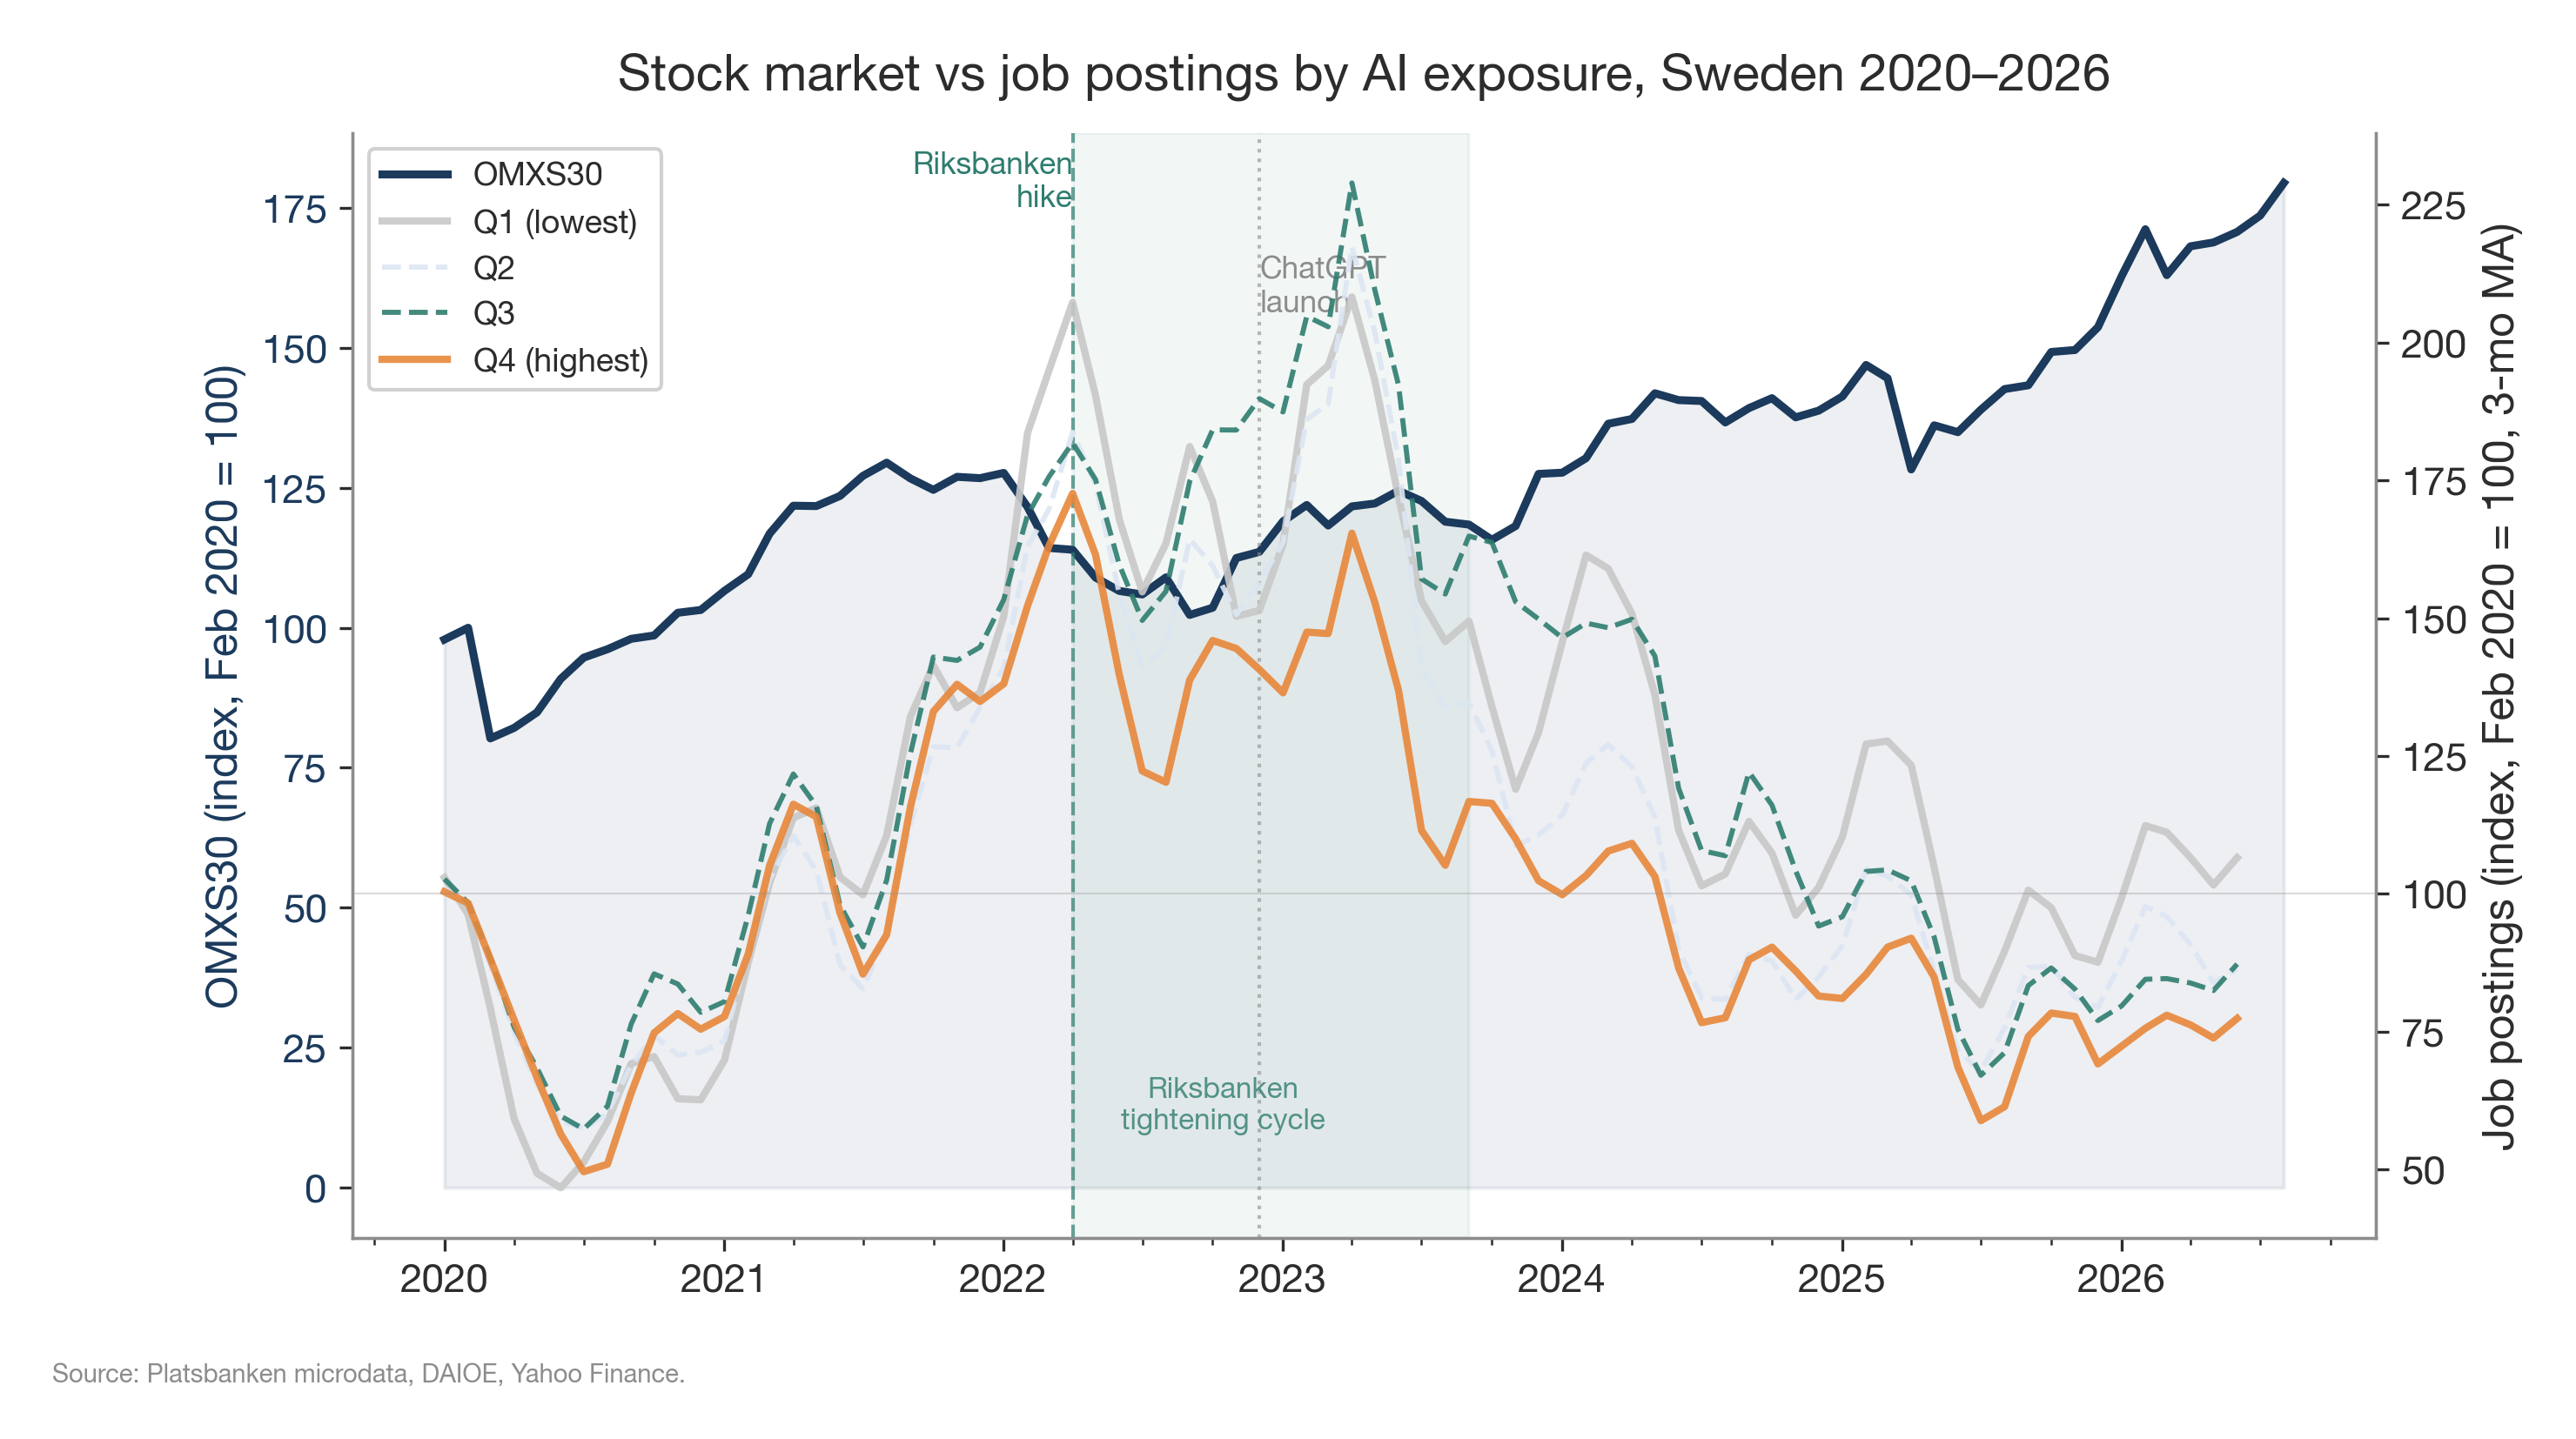
\includegraphics[width=\textwidth]{fig1_scary_chart.png}
\end{column}
\end{columns}
\end{frame}

% ============================================================
% MOTIVATION: WHAT WE KNOW
% ============================================================
\begin{frame}{What do we know about GenAI and employment?}
\begin{itemize}
    \item \textbf{Brynjolfsson et al.\ (2025):} 16\% relative employment decline for young workers in AI-exposed fields
    \item \textbf{Humlum \& Vestergaard (2025):} null on Danish earnings; borderline hiring decline for 22--25
    \item \textbf{Kauhanen \& Rouvinen (2025, 2026):} null in Finland (synthetic DiD)
    \item \textbf{Teutloff, Kässi et al.\ (2025):} 20--50\% decline in substitutable freelance skills
\end{itemize}
\vspace{2mm}
\begin{block}{Our contribution}
\begin{enumerate}
    \item Reconcile aggregate decline (macro) with compositional shift (AI)
    \item Exploit Sweden's 7-month gap between rate hike and ChatGPT as timing test
\end{enumerate}
\end{block}
\end{frame}

% ============================================================
% MOTIVATION: WHAT WE KNOW
% ============================================================
\begin{frame}{What do we know about gender differences?}
\begin{itemize}
    \item \textbf{{Brynjolfsson et al.\ (2025):}} find similar trends for men and women, with a slightly larger decline for young women in exposed professions.
    \item \textbf{{Cazzaniga et al.\ (2025):}} a higher share of women than men work in AI exposed occupations which makes them more likely to be affected.
    \item \textbf{{Gardberg et al.\ (2025):}} simulations indicate that the gender wage gap may widen in many scenarios, as women are disproportionately represented in highly exposed occupations.
\end{itemize}
\vspace{2mm}
\begin{block}{Our contribution}
\begin{enumerate}
    \item Population-register evidence on gender differences in development in \textit{employment} since launch of ChatGPT
\end{enumerate}
\end{block}
\end{frame}



\section{Data and Identification}

% ============================================================
% DATA
% ============================================================
\begin{frame}{Two margins of analysis}
\begin{columns}[T]
\begin{column}{0.48\textwidth}
\begin{block}{Posting margin}
\begin{itemize}
    \item \textbf{Platsbanken} (AF): 4.6M ads, 2020--2026
    \item Matched to SSYK 4-digit occupations
    \item AI exposure via DAIOE quartiles
    \item Timing test: Riksbank hike vs ChatGPT
\end{itemize}
\end{block}
\end{column}
\begin{column}{0.48\textwidth}
\begin{block}{Employment margin}
\begin{itemize}
    \item \textbf{AGI register}: full population, monthly, employer-employee linked
    \item Six age groups: 22--25 through 50+
    \item Within-employer DiD design
    \item Question: does the \textit{age composition} shift?
\end{itemize}
\end{block}
\end{column}
\end{columns}
\vspace{5mm}
\begin{center}
\textit{In this presentation I will focus on the employment margin}
\end{center}
\end{frame}

% ============================================================
% DAIOE: AI EXPOSURE MEASURE
% ============================================================
\begin{frame}{Measuring AI exposure: DAIOE}
\begin{columns}[T]
\begin{column}{0.55\textwidth}
\textbf{DAIOE} (Engberg et al.\ 2024, IZA DP 16717)
\begin{enumerate}
    \item Start from 52 AI capabilities (what current AI systems can do)
    \item Match capabilities to O*NET cognitive ability ratings
    \item Aggregate ability-level scores to occupations
    \item Map to Swedish occupations: SOC $\to$ ISCO $\to$ SSYK
\end{enumerate}
\vspace{2mm}
\begin{itemize}
    \item Captures \textit{what AI can do}, not whether firms have adopted
    \item GenAI-specific variant isolates generative AI capabilities
    \item Cross-validated: Eloundou et al.\ (2024), Pulito et al.\ (2026)
\end{itemize}
\end{column}
\begin{column}{0.42\textwidth}
\begin{block}{High exposure (Q4)}
\footnotesize
Customer service, payroll administrators, receptionists, software developers, bookkeepers, secretaries
\end{block}
\vspace{2mm}
\begin{block}{Low exposure (Q1)}
\footnotesize
Construction workers, vehicle drivers, cleaners, childcare workers, chefs, nurses
\end{block}
\end{column}
\end{columns}
\hypertarget{main:daioe}{}
\end{frame}

% ============================================================
% DATA: REGISTER DATA DEEP DIVE
% ============================================================
\begin{frame}{Register data: AGI}
\begin{columns}[T]
\begin{column}{0.55\textwidth}
\textbf{Arbetsgivardeklarationen (AGI)}
\begin{itemize}
    \item Monthly employer declarations to Skatteverket
    \item Administrative population data --- every employee, every employer
    \item Individual-level since January 2019
    \item SSYK 2012 at 4-digit level (from 2023)
    \item Employer-employee link: who works where, when
\end{itemize}
\vspace{2mm}
\textbf{What this enables:}
\begin{itemize}
    \item Within-employer analysis (not possible with surveys)
    \item Monthly dynamics (not annual snapshots)
    \item No sampling error
\end{itemize}
\end{column}
\begin{column}{0.42\textwidth}
\begin{block}{Panel dimensions}
\footnotesize
\begin{tabular}{ll}
Employers & 510,213 \\
& {\tiny (with $\geq$1 SSYK-coded} \\
& {\tiny employee)} \\
Age groups & 6 \\
AI quartiles & 4 \\
Months & 73 \\
Non-zero cells & 75M \\
\end{tabular}
\end{block}
\end{column}
\end{columns}
\end{frame}

% ============================================================
% IDENTIFICATION: EMPLOYMENT MARGIN
% ============================================================
\begin{frame}{Identification: employment margin}
\textbf{Employer-level DiD} (following Brynjolfsson et al.\ 2025):
\vspace{-2mm}
\begin{equation*}
\ln E_{j,q,t}^{a} = \gamma_1 (\text{PostRB}_t \times Q4_q) + \gamma_2 (\text{PostGPT}_t \times Q4_q ) + \delta_{j,q} + \delta_{j,t} + \varepsilon_{j,q,t}
\end{equation*}

\begin{itemize}
    \item $\delta_{j,q}$: employer $\times$ quartile FE --- absorbs permanent employer-occupation composition
    \item $\delta_{j,t}$: employer $\times$ month FE --- absorbs \textbf{all time-varying employer shocks}
    \item[$\Rightarrow$] Identification: \textit{within the same employer, in the same month}, do workers in high-AI occupations shift differently by age?
    \item Separate regressions for each age group and gender
\end{itemize}
\vspace{2mm}
\begin{alertblock}{What employer $\times$ month FE absorbs}
All time-varying employer-level shocks: hiring freezes, downsizing, industry cycles, regional shocks, seasonal patterns. Remaining variation: \textit{within}-employer shifts across AI exposure quartiles, by age.
\end{alertblock}
\end{frame}

\section{Results}

% ============================================================
% RESULT 1: POSTING MARGIN
% ============================================================
\begin{frame}{Result 1: posting decline is monetary, not AI}
\begin{columns}[c]
\begin{column}{0.55\textwidth}
\begin{itemize}
    \item $\hat{\beta}_1$ (PostRB $\times$ High) $= -0.127$, $p < 0.01$
    \item $\hat{\beta}_2$ (PostGPT $\times$ High) $= -0.062$, $p = 0.11$
    \item Divergence opens with monetary tightening, not ChatGPT
\end{itemize}
\vspace{3mm}
\textbf{Robustness:}
\begin{itemize}
    \item Negative in 7/8 specifications, significant in 2
    \item Teleworkability split: zero effect in teleworkable occupations; $\beta_2 = -0.233$ ($p < 0.01$) in non-teleworkable
\end{itemize}
\end{column}
\begin{column}{0.43\textwidth}
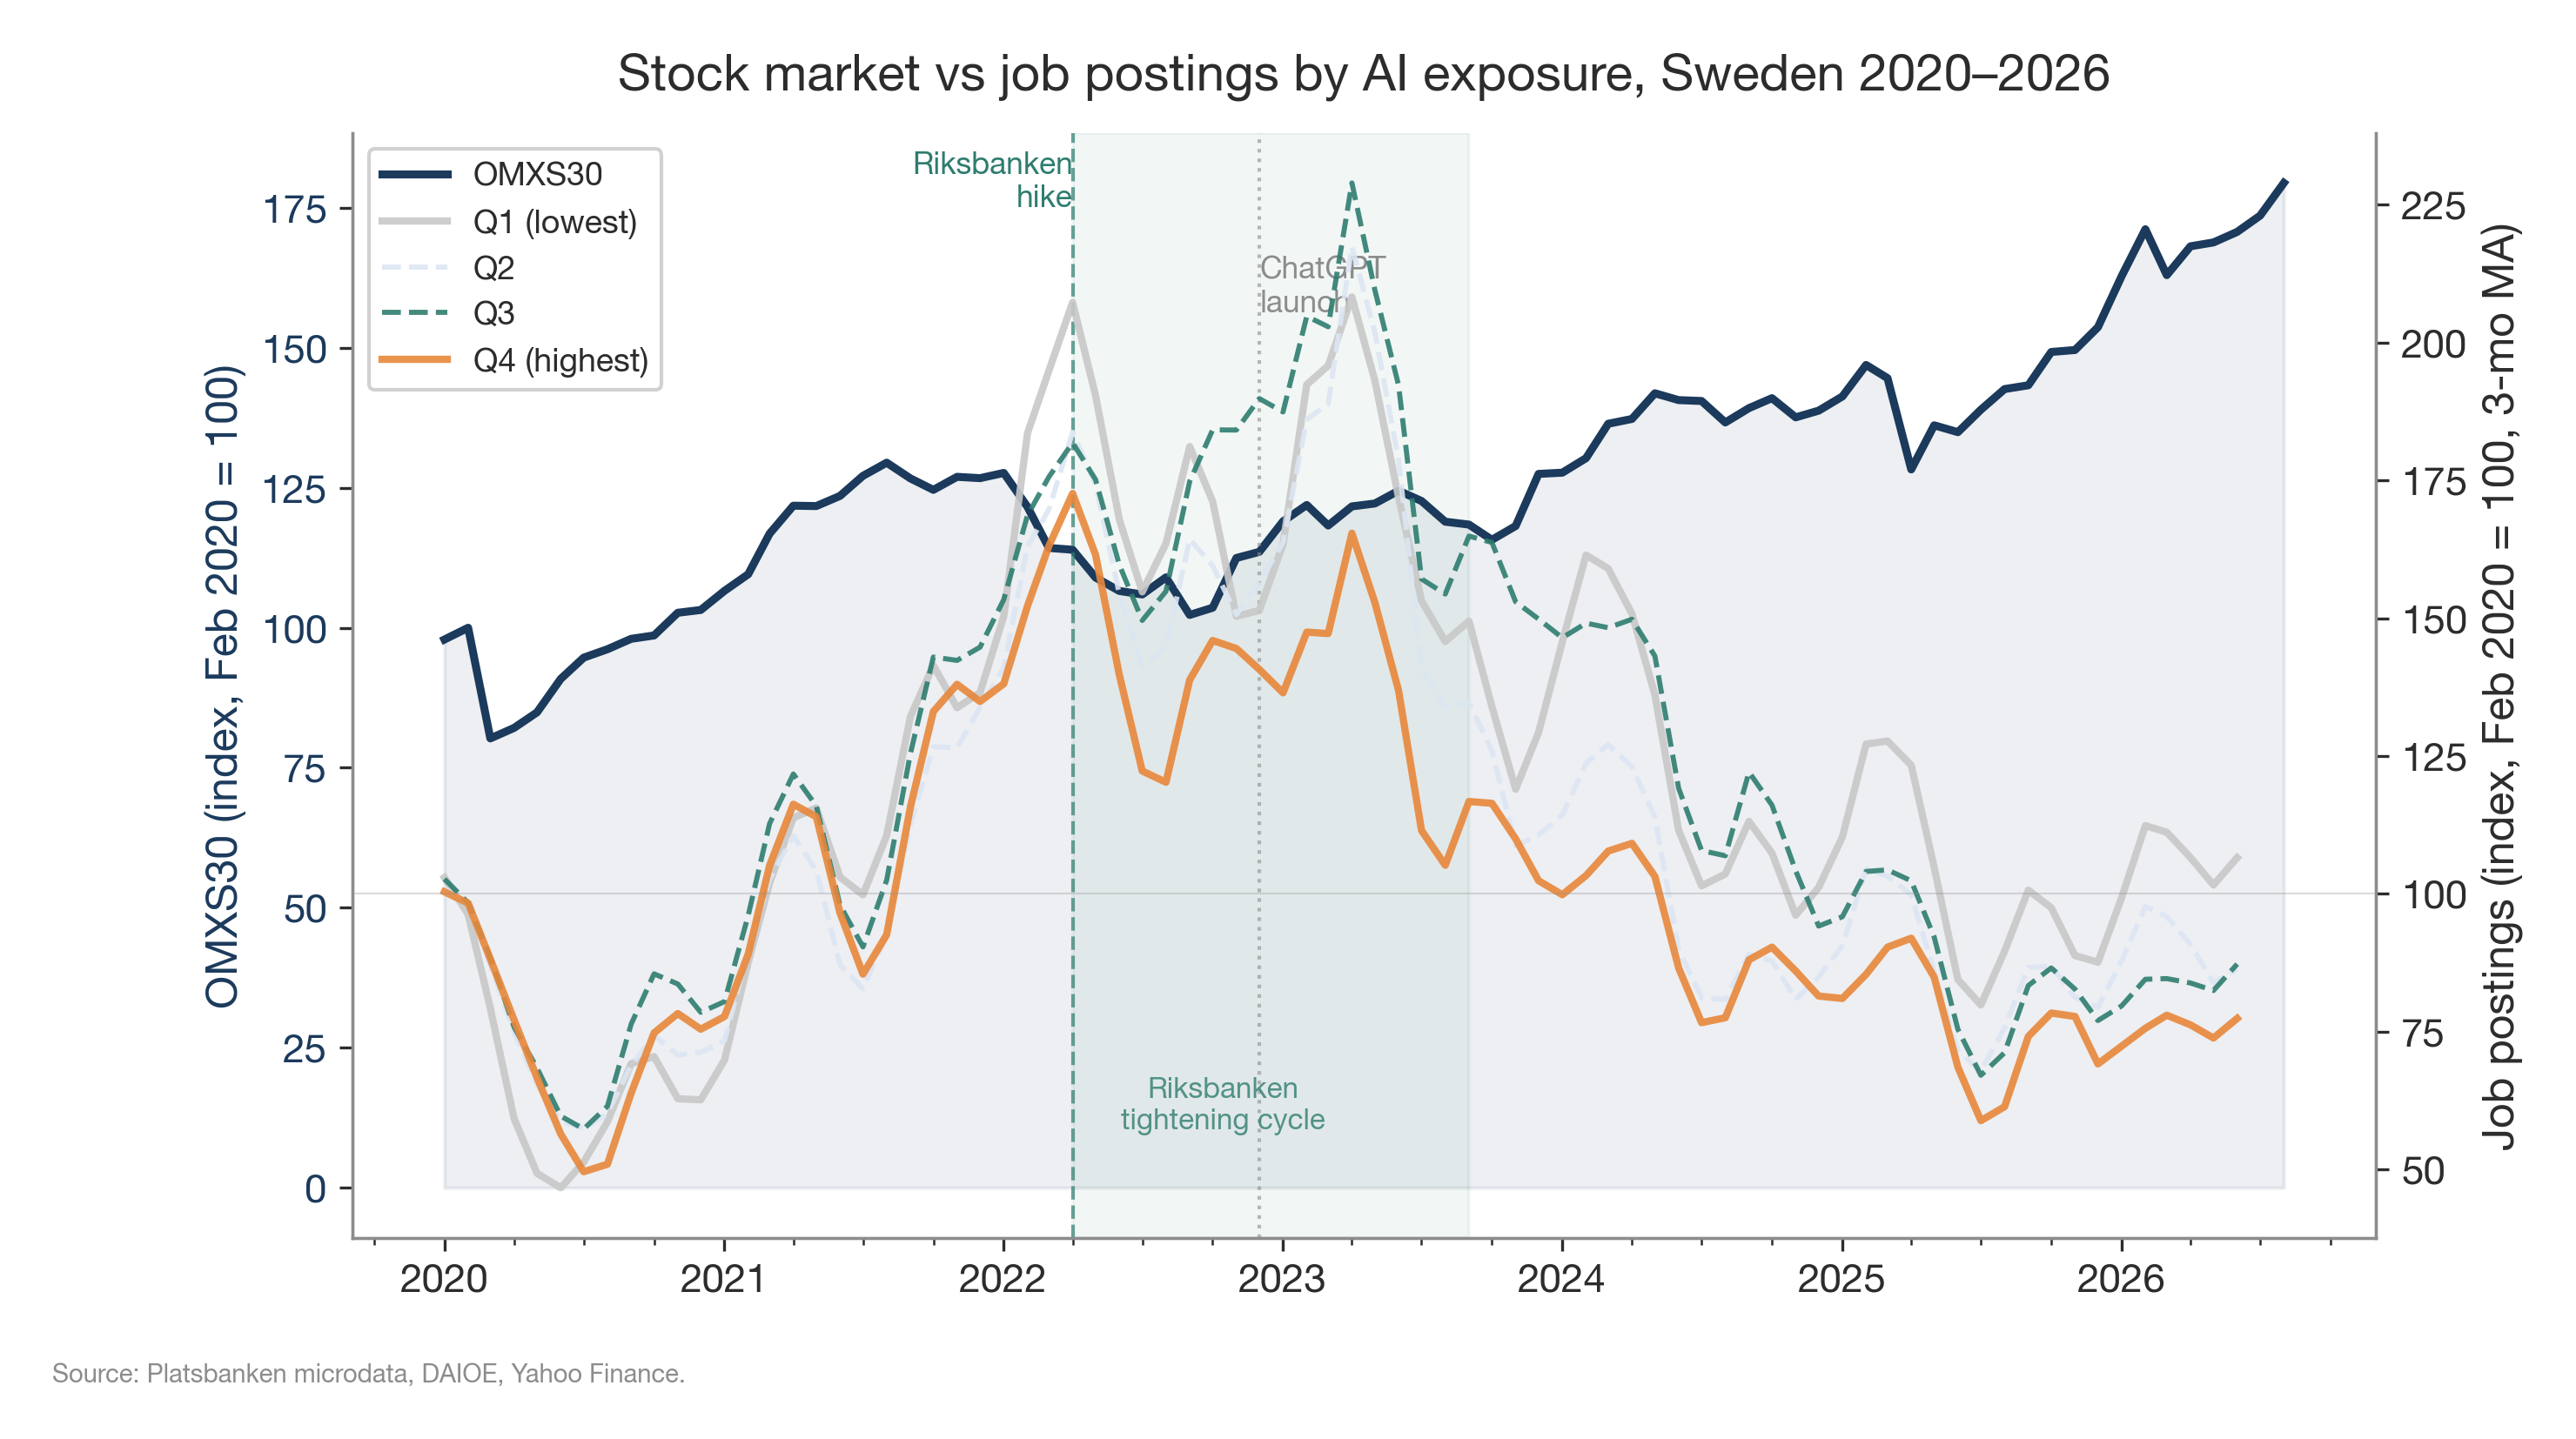
\includegraphics[width=\textwidth]{fig1_scary_chart.png}\\[2mm]
\footnotesize \textit{Posting indices (Feb 2020 = 100) by DAIOE quartile, with OMXS30 and policy rate timeline}
\end{column}
\end{columns}
\end{frame}

% ============================================================
% RESULT 2: CANARIES
% ============================================================
\begin{frame}{Result 2: young workers are the ``canaries''}
\begin{columns}[c]
\begin{column}{0.48\textwidth}
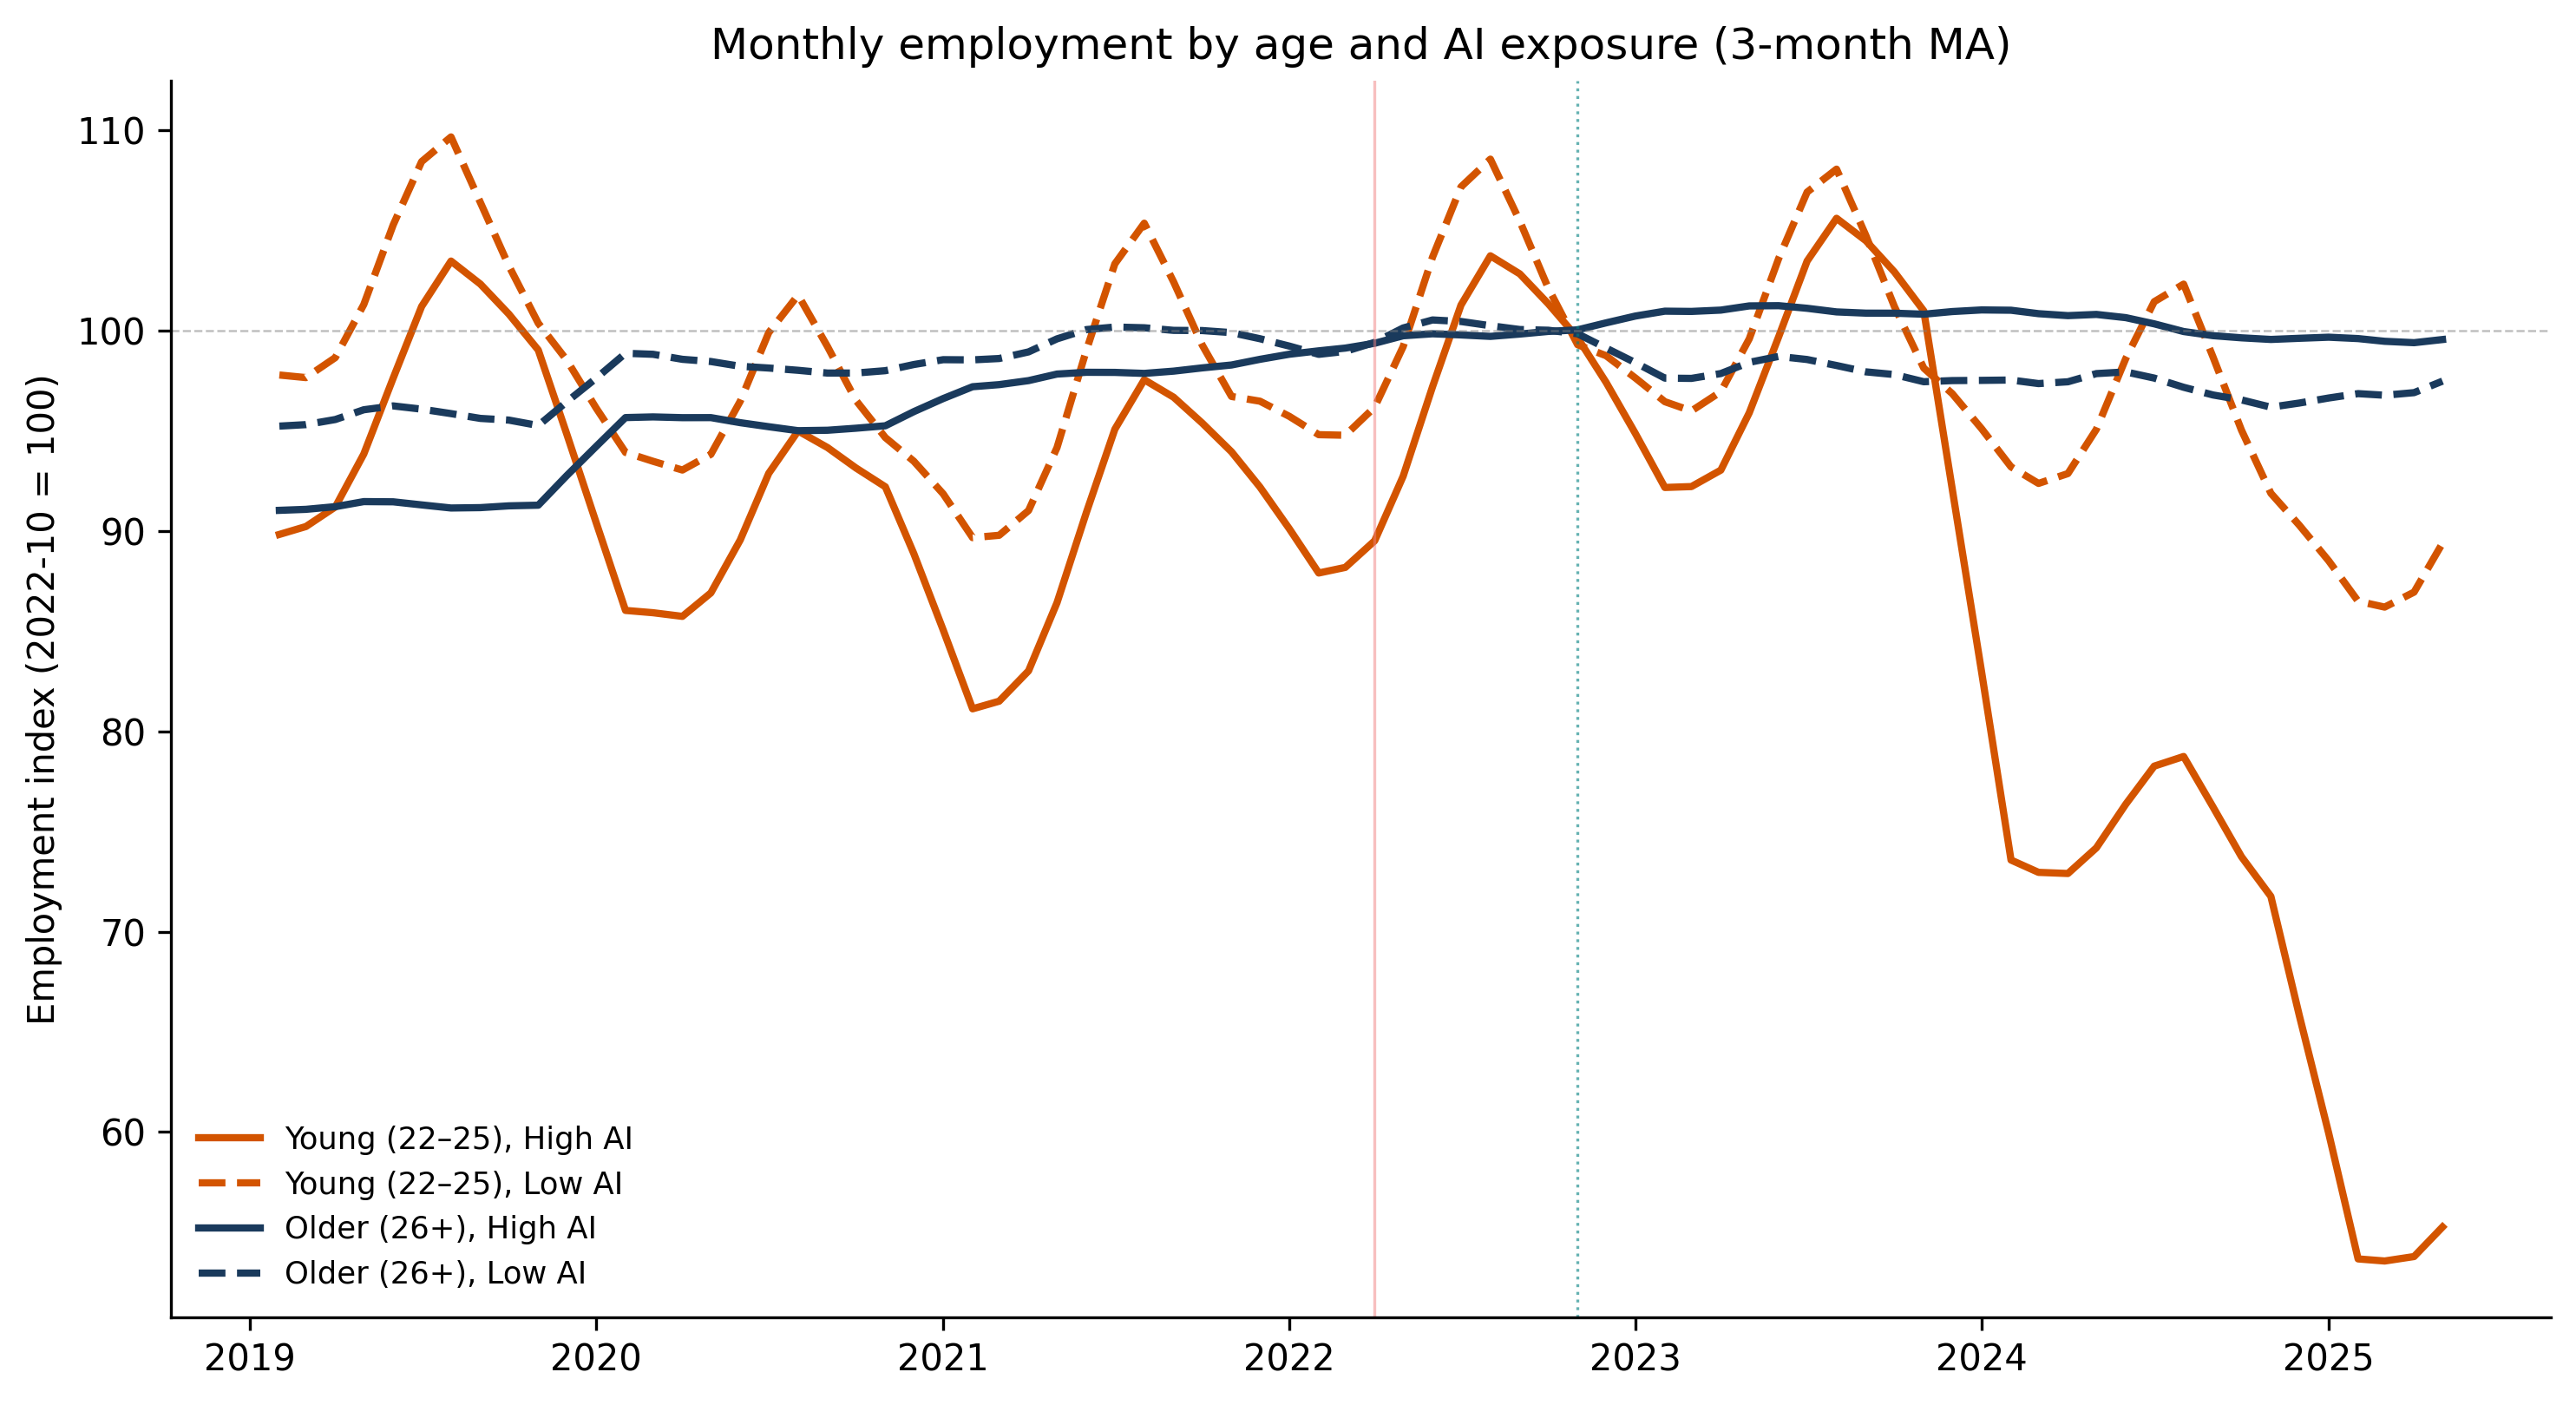
\includegraphics[width=\textwidth]{fig2_mona_canaries_ma3.png}
\end{column}
\begin{column}{0.48\textwidth}
\begin{itemize}
    \item Within the \textbf{same employers}: employment of 22--25-year-olds in high-AI occupations diverges sharply after ChatGPT
    \item Gap widens through 2024--2025
    \item Workers 50+ show \textit{opposite} pattern: rising in high-AI occupations
    \item[$\Rightarrow$] Compositional shift, not aggregate destruction
\end{itemize}
\vspace{2mm}
\footnotesize
\textit{Residualised employment gap (Q4 minus Q1--Q3) within employers, 3-month MA. Full-population AGI data.}\\[1mm]
{\tiny\hyperlink{backup:spotlight}{\beamergotobutton{Spotlight occupations}}}
\end{column}
\end{columns}
\end{frame}

% ============================================================
% RESULT 3: EVENT STUDY
% ============================================================
\begin{frame}{Result 3: accelerating age gradient}
\begin{columns}[c]
\begin{column}{0.48\textwidth}
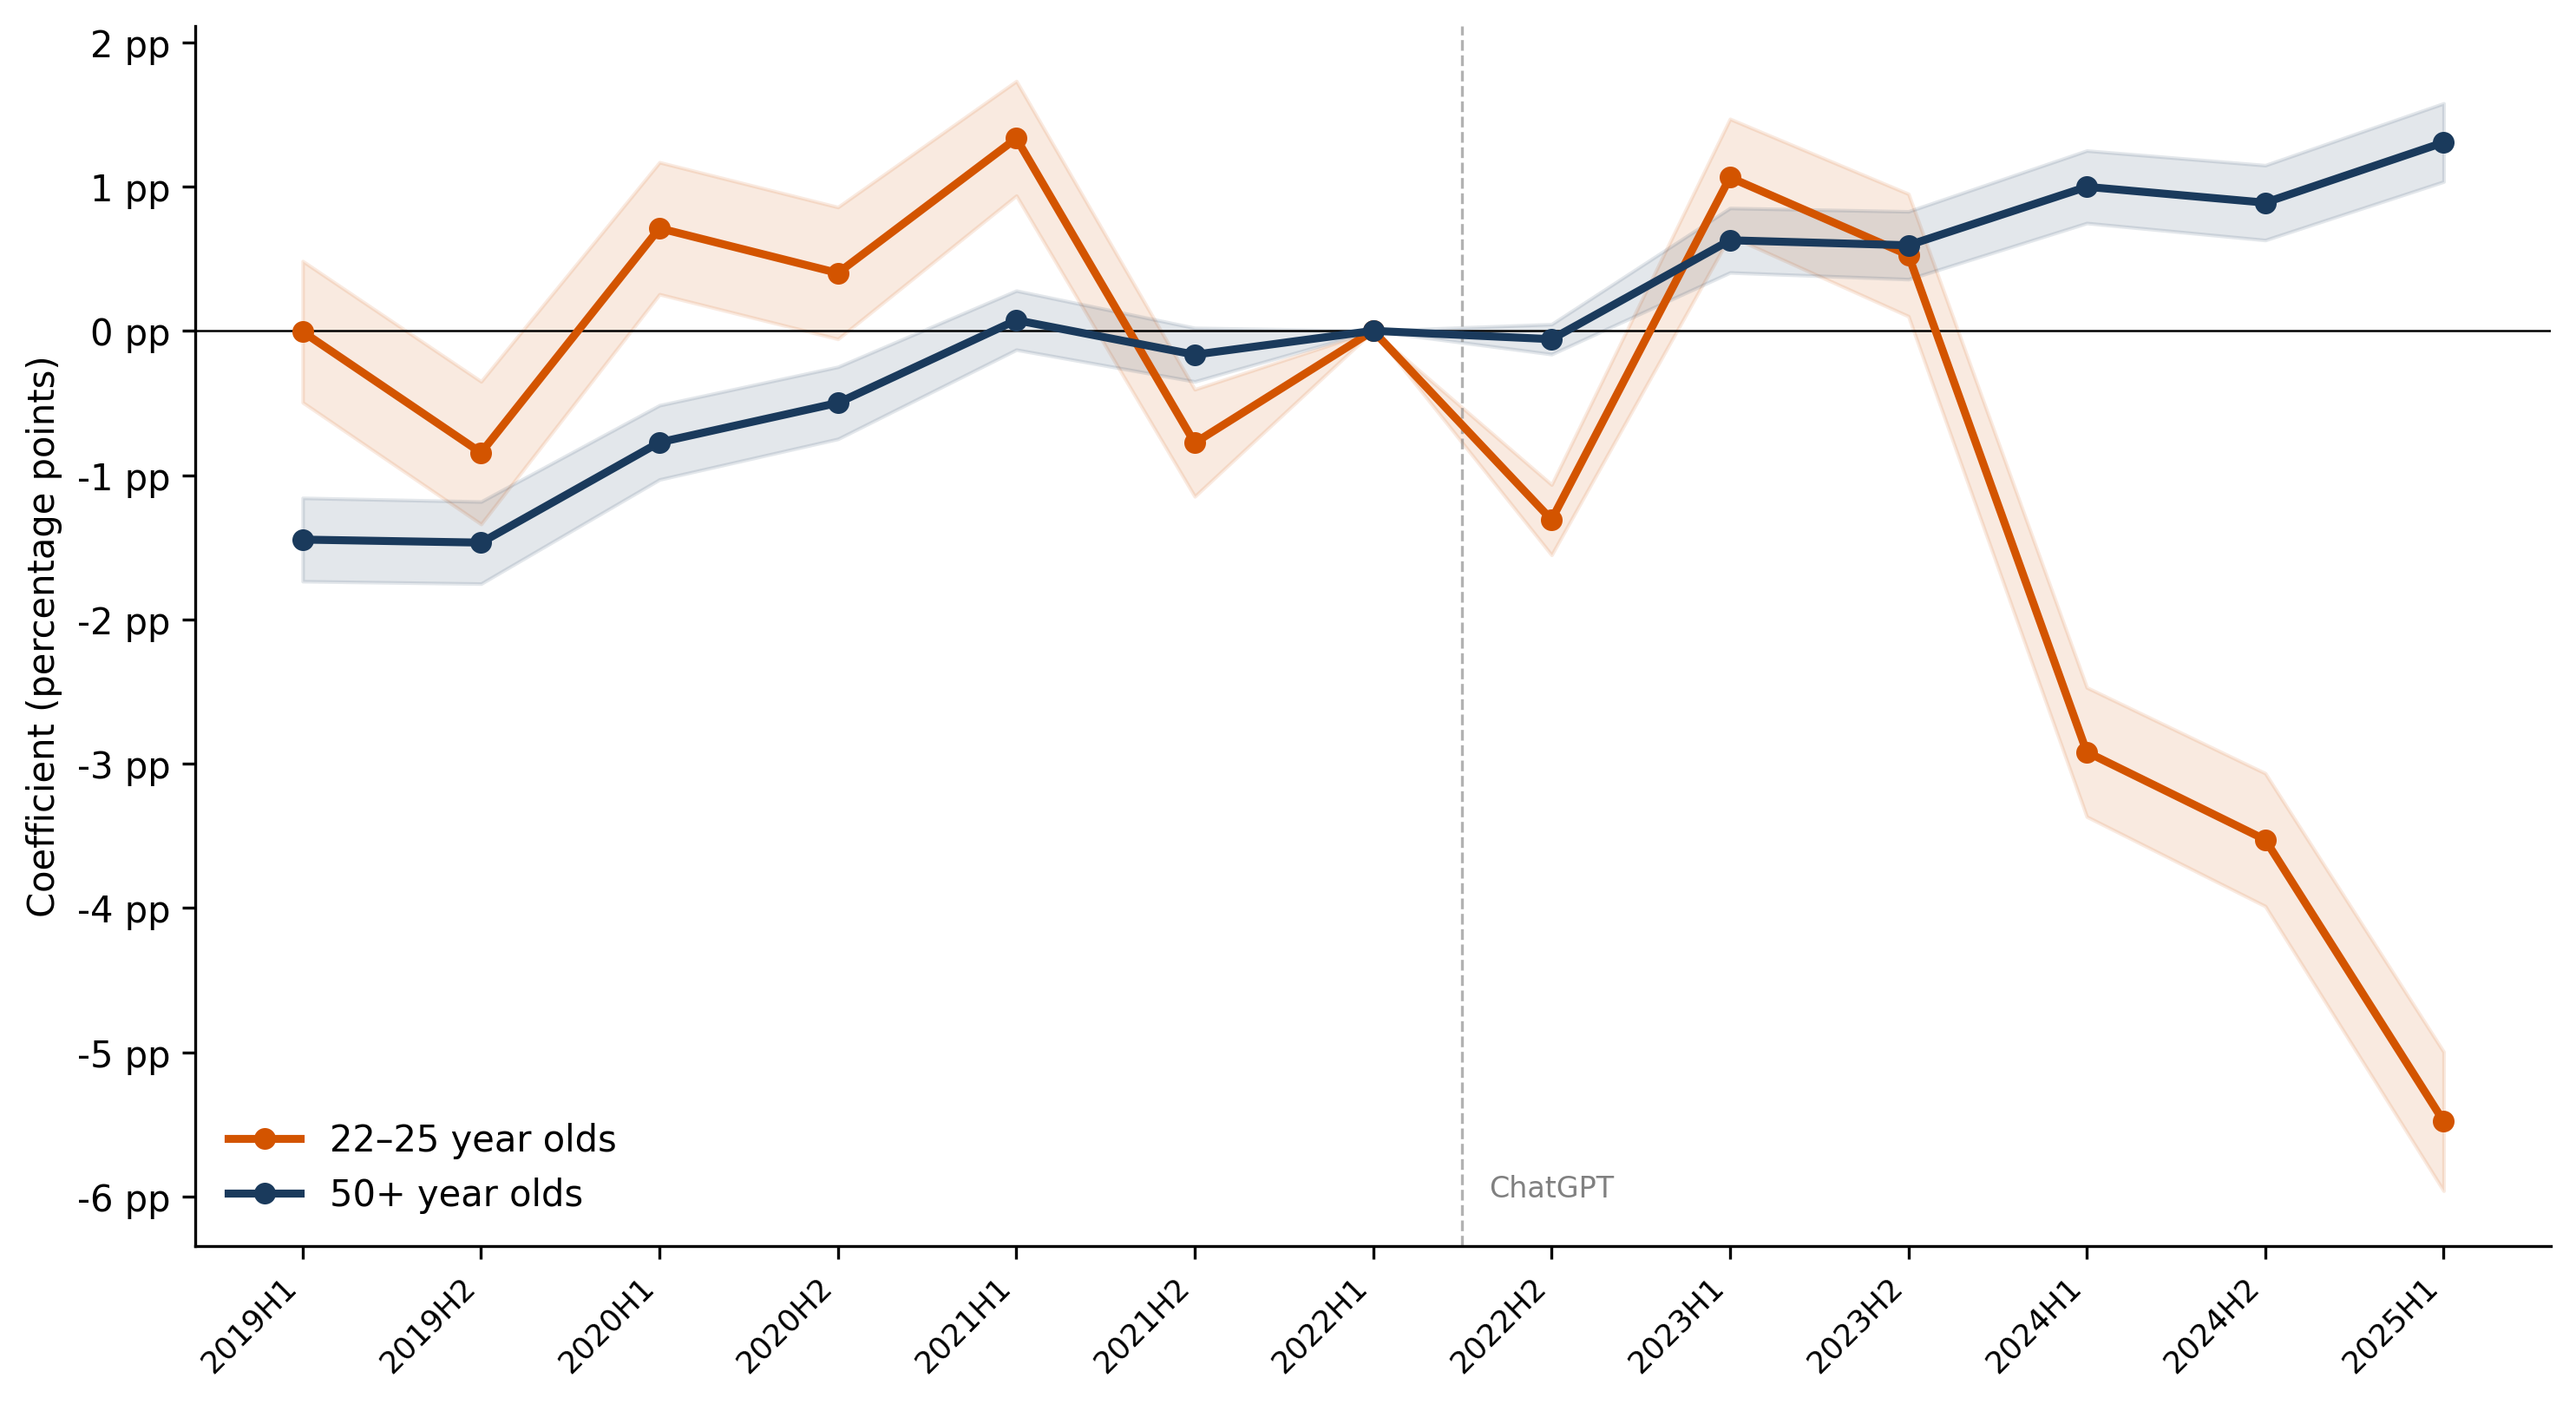
\includegraphics[width=\textwidth]{fig3_event_study_main.png}
\end{column}
\begin{column}{0.50\textwidth}
\textbf{Key numbers:}
\begin{itemize}
    \item 22--25 in Q4: $-5.5\%$ by early 2025
    \item 26--30 in Q4: $-4.9\%$ by early 2025
    \item 50+ in Q4: $+1.3\%$
\end{itemize}
\vspace{3mm}
\textbf{Consistent with Brynjolfsson et al.\ (2025):}
\begin{itemize}
    \item US: 16\% decline (ADP payroll, 25M+ workers)
    \item Sweden: 5.5\% (AGI register, full population)
    \item Both within-employer, same direction
    \item Differs from Danish and Finnish findings
\end{itemize}
\vspace{2mm}
\end{column}
\end{columns}
\end{frame}

\section{Interpretation}


% ============================================================
% INTERPRETATION
% ============================================================
\begin{frame}{Interpretation: task-based framework}
\begin{center}
\resizebox{0.8\textwidth}{!}{
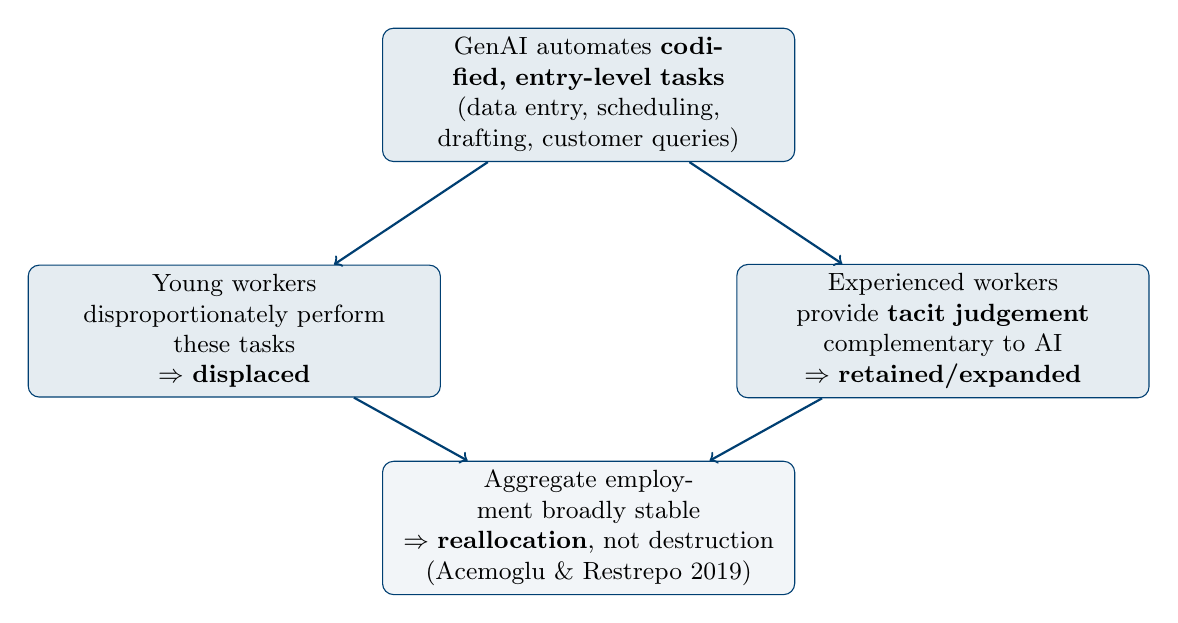
\begin{tikzpicture}[
    box/.style={rectangle, draw=oruBlue, fill=oruBlue!10, rounded corners, text width=5cm, minimum height=1.2cm, align=center, font=\small},
    arrow/.style={->, thick, oruBlue}
]
\node[box] (ai) at (0,3) {GenAI automates \textbf{codified, entry-level tasks}\\(data entry, scheduling, drafting, customer queries)};
\node[box] (young) at (-4.5,0) {Young workers\\disproportionately perform\\these tasks\\$\Rightarrow$ \textbf{displaced}};
\node[box] (old) at (4.5,0) {Experienced workers\\provide \textbf{tacit judgement}\\complementary to AI\\$\Rightarrow$ \textbf{retained/expanded}};
\node[box, fill=oruBlue!5] (net) at (0,-2.5) {Aggregate employment broadly stable\\$\Rightarrow$ \textbf{reallocation}, not destruction\\(Acemoglu \& Restrepo 2019)};
\draw[arrow] (ai) -- (young);
\draw[arrow] (ai) -- (old);
\draw[arrow] (young) -- (net);
\draw[arrow] (old) -- (net);
\end{tikzpicture}
}
\end{center}

\vspace{2mm}
{\footnotesize \textit{Slight caveat: Swedish employment protection law protects senior workers — cannot
fully disentangle from AI complementarity.}}
\end{frame}


% ============================================================
% GENDER
% ============================================================

\begin{frame}{Gender heterogeneity}
\centering

\begin{table}[htbp]
\centering
\caption{Employment distribution by AI exposure and gender (ages 22--25, full sample)}
\label{tab:ai_exposure_gender_full}
\begin{tabular}{llcccc}
\toprule
Period & Gender & High AI (Q4) & Low AI (Q1--Q3) & Total & Share Q4 (\%) \\
\midrule
\multirow{Base (2022-10)} 
 & Men   & 657,510 & 1,881,204 & 2,538,714 & 25.90 \\
 & Women & 765,533 & 1,694,078 & 2,459,611 & 31.12 \\
\midrule
\multirow{Latest (2025-06)} 
 & Men   & 648,332 & 1,820,761 & 2,469,093 & 26.26 \\
 & Women & 756,708 & 1,719,810 & 2,476,518 & 30.56 \\
\bottomrule
\end{tabular}

\begin{flushleft}
\footnotesize \textit{Shares are calculated within gender. Women are consistently more concentrated in high-AI occupations than men, although the share declines slightly over time.}
\end{flushleft}

\end{table}
\end{frame}

\begin{frame}{Gender heterogeneity}
\centering

Effect roughly \textbf{twice as large for young women} ($\hat{\gamma}_2 = -0.016$) as for young men ($-0.007$) but...

\vspace{3mm}

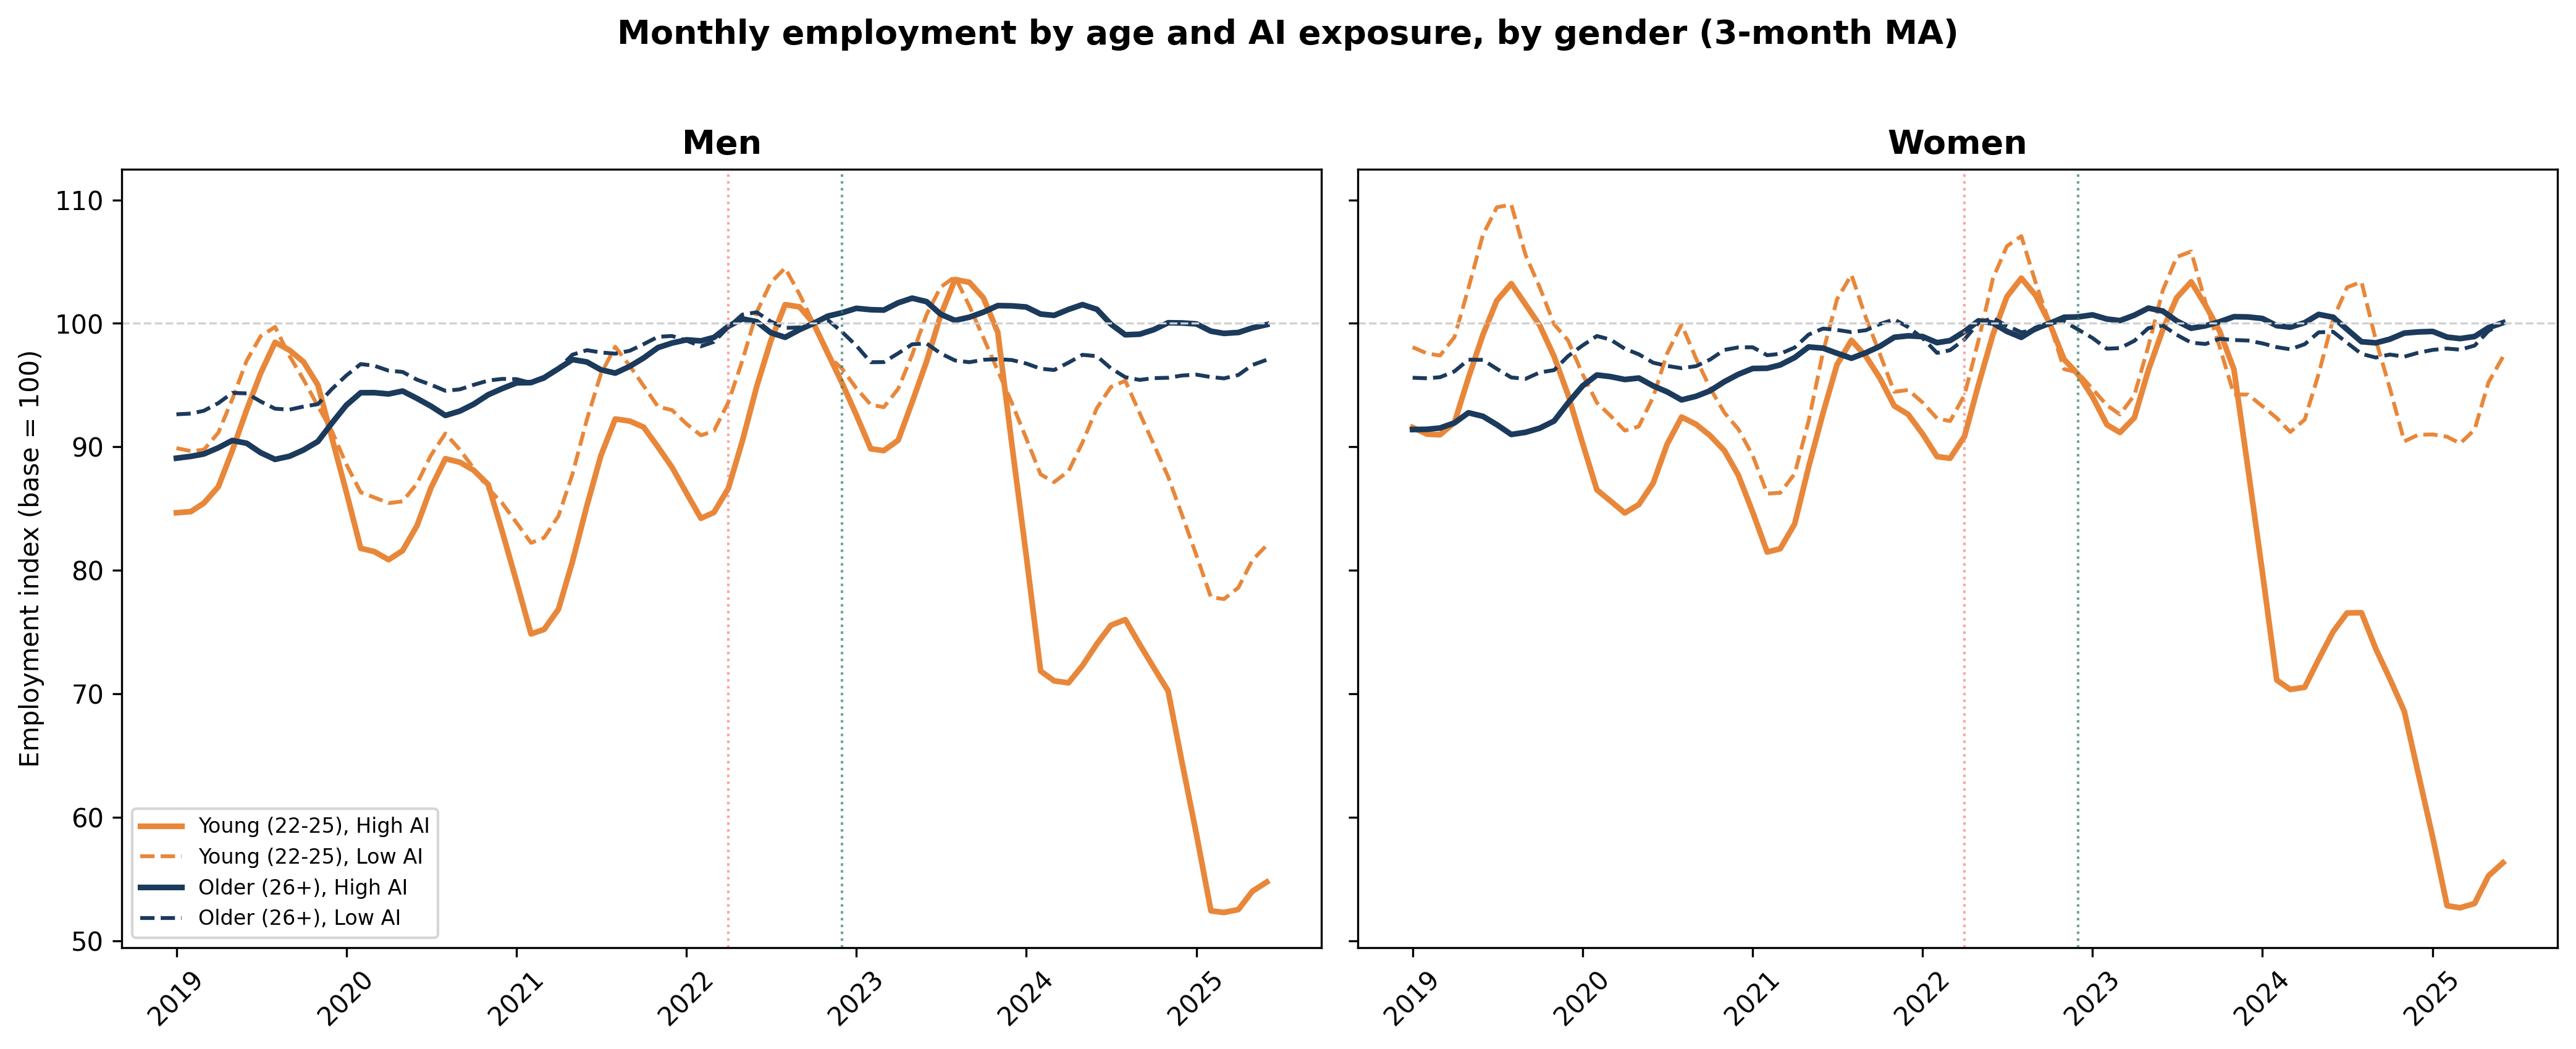
\includegraphics[width=0.9\textwidth]{figA_gender_canaries_panel_corrected.png}
\end{frame}

\begin{frame}{Gender heterogeneity}
\begin{itemize}
    \item Labour outcomes for men in low AI-exposure occupations have declined more than for women in the same occupations. This makes the relative difference larger for women. 
    \item To investigate whether this can be explained by the fact that women and men sort into different occupations, we apply an Oaxaca-Blinder-style re-weighting decomposition
    \item We re-estimate the women’s regressions using inverse probability weights (IPW) that adjust women’s occupational distribution within Q4 to match men’s. If the gender gap narrows after reweighting, the between-occupation (composition) component is a contributing factor; if the gap persists, the within-occupation (coefficient) component dominates.
\end{itemize}
\vspace{2mm}
\end{frame}

\begin{frame}{Gender heterogeneity}
\begin{itemize}
\item The reweighting shows that occupational composition explains $\sim$1/3 of the gap
    \item Remaining 2/3 is \textbf{within-occupation}
    \item For 41--49 women: entire negative effect disappears after reweighting
    \item Points to more adverse effects in female-dominated occupations
    \end{itemize}

\end{frame}


\section{Conclusion}

% ============================================================
% CONCLUSION AND POLICY
% ============================================================
\begin{frame}{Conclusions and policy implications}
\begin{columns}[T]
\begin{column}{0.48\textwidth}
\textbf{Findings}
\begin{enumerate}
    \item Aggregate posting decline $=$ monetary tightening
    \item Compositional employment shift $=$ AI
    \item Young workers in AI-exposed occupations: $-5.5\%$ by early 2025 (accelerating)
    \item Older workers: $+1.3\%$
    \item Young women in AI-exposed fields face a twice as large \textit{relative} decline
    \item Women overrepresented in highly exposed occupations that face employment declines 
\end{enumerate}
\end{column}
\begin{column}{0.48\textwidth}
\textbf{Policy relevance}
\begin{itemize}
    \item Early-career workers in AI-exposed occupations need targeted support
    \item Transition pathways: redesign of entry-level roles
\end{itemize}
\end{column}
\end{columns}
\vspace{2mm}
\begin{center}
\large\textcolor{oruBlue}{Thank you! Questions?}\\[1mm]
\scriptsize lydia.lothman@oru.se
\end{center}
\end{frame}

% ============================================================
% BACKUP SLIDES
% ============================================================
\appendix


% ============================================================
% PLACEBO AND PRE-TRENDS
% ============================================================

\begin{frame}[plain]
\begin{center}
\vspace{2cm}
{\Large\textcolor{oruBlue}{Backup Slides}}
\end{center}
\end{frame}

\begin{frame}{Robustness: placebo and pre-trends}
\begin{columns}[c]
\begin{column}{0.48\textwidth}
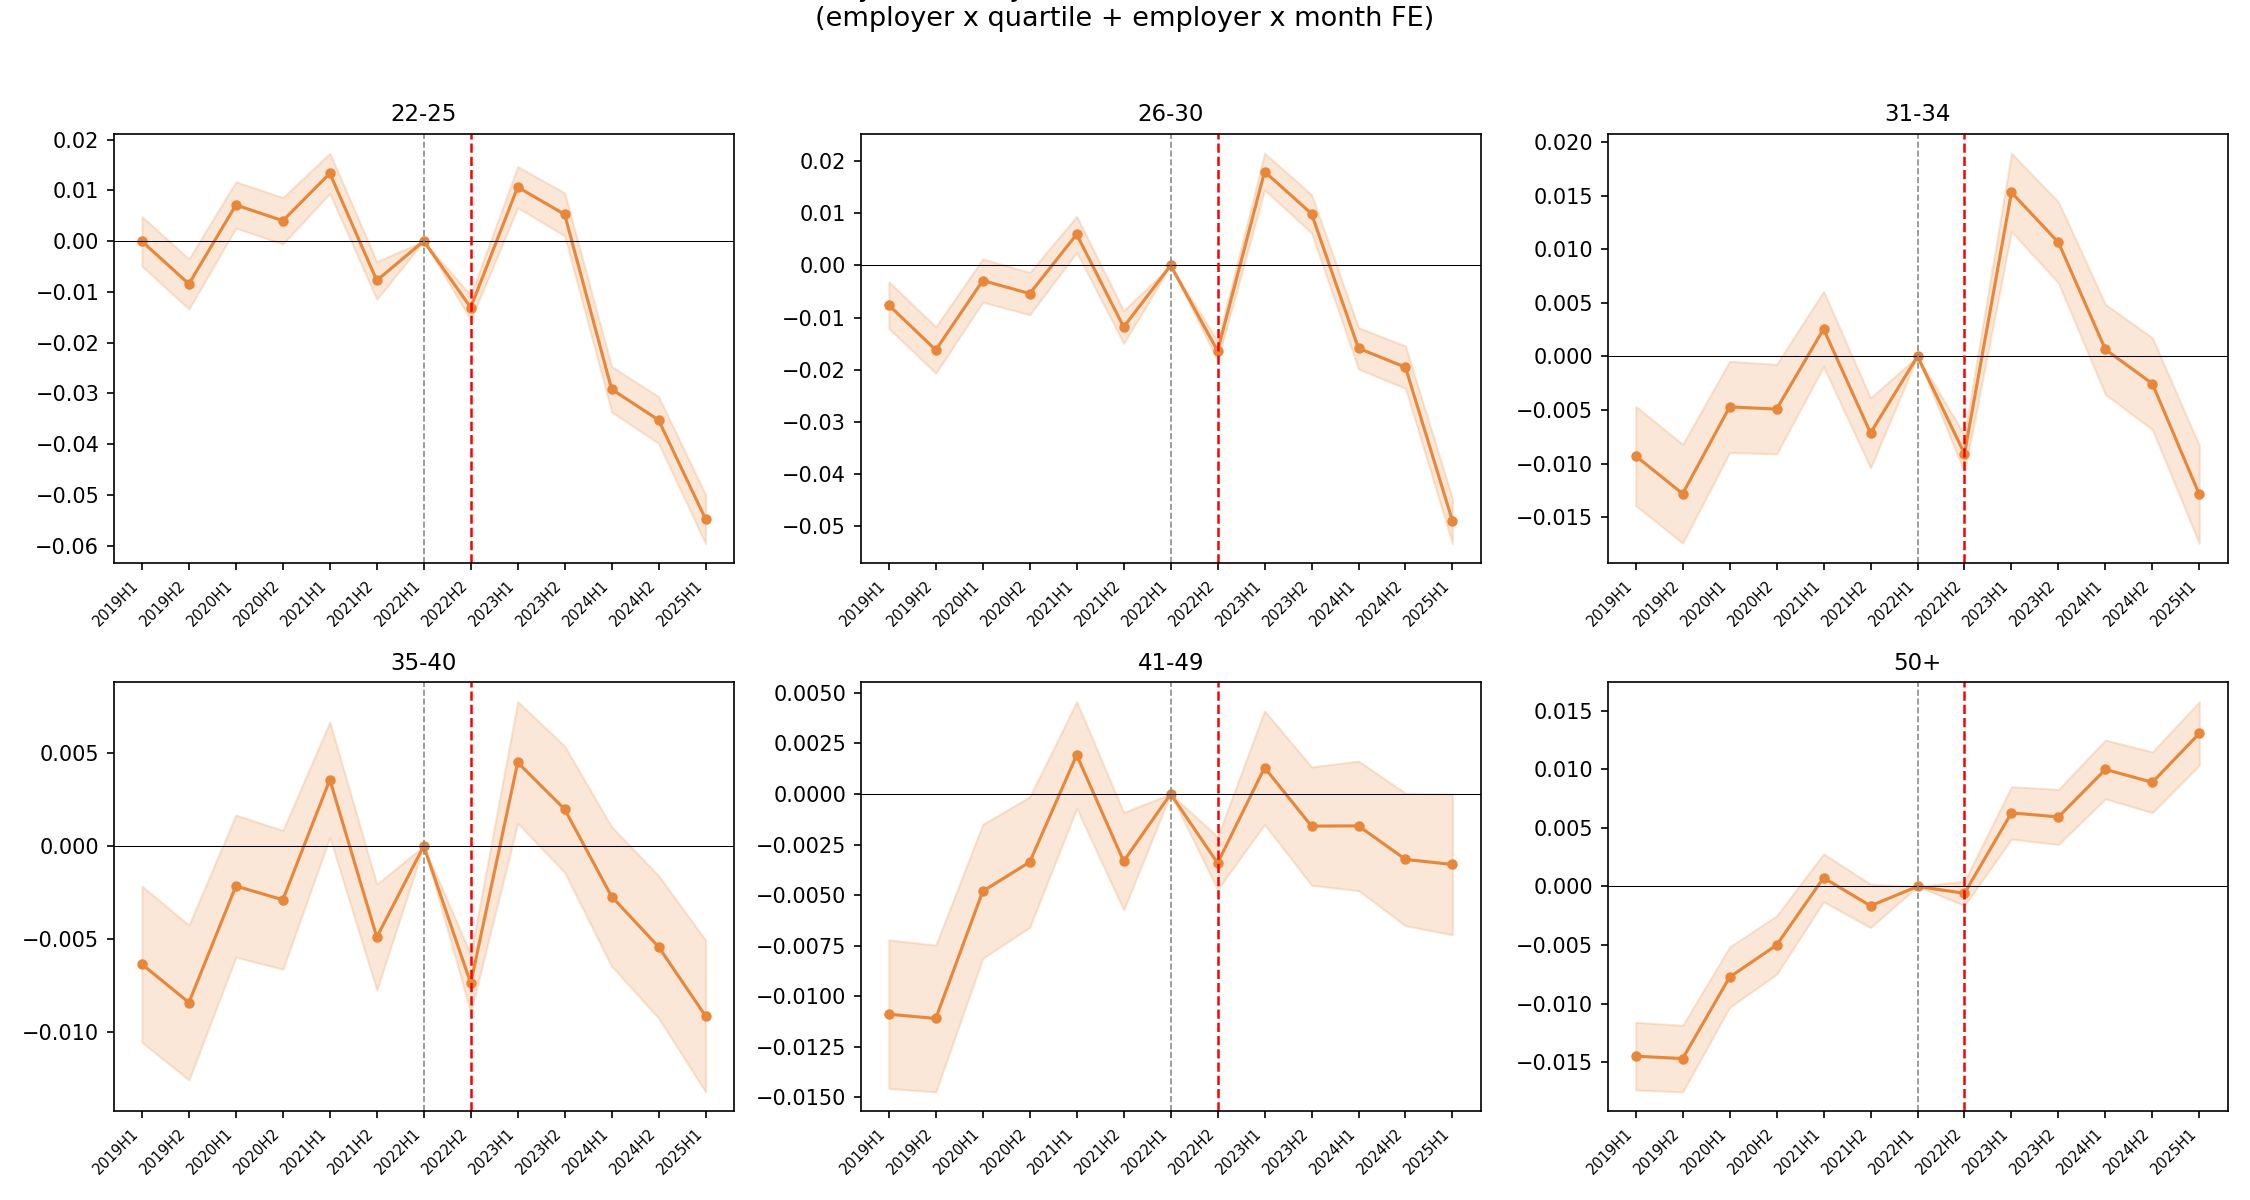
\includegraphics[width=\textwidth]{placebo_jul2022_es_panel.png}\\
\footnotesize \textit{Placebo: July 2022 treatment date}
\end{column}
\begin{column}{0.50\textwidth}
\textbf{Placebo test (July 2022):}
\begin{itemize}
    \item Flat through 2023
    \item Sharp acceleration only in 2024--2025
    \item Inconsistent with pre-existing trends
\end{itemize}
\vspace{3mm}
\textbf{Pre-trend assessment:}
\begin{itemize}
    \item Pre-trend tests reject for all age groups (Roth 2022)
    \item But: slopes are \textit{positive} for young workers --- works \textit{against} our finding
    \item Cumulative pre-trend bias for 22--25: $+0.004$ vs endpoint $-0.055$ (7\%, wrong direction)
    \item Rambachan-Roth: average effects fragile (dilution of late-period signal)
\end{itemize}
\end{column}
\end{columns}
\end{frame}




\begin{frame}{Spotlight: four AI-exposed occupations}
\hypertarget{backup:spotlight}{}
\begin{columns}[c]
\begin{column}{0.48\textwidth}
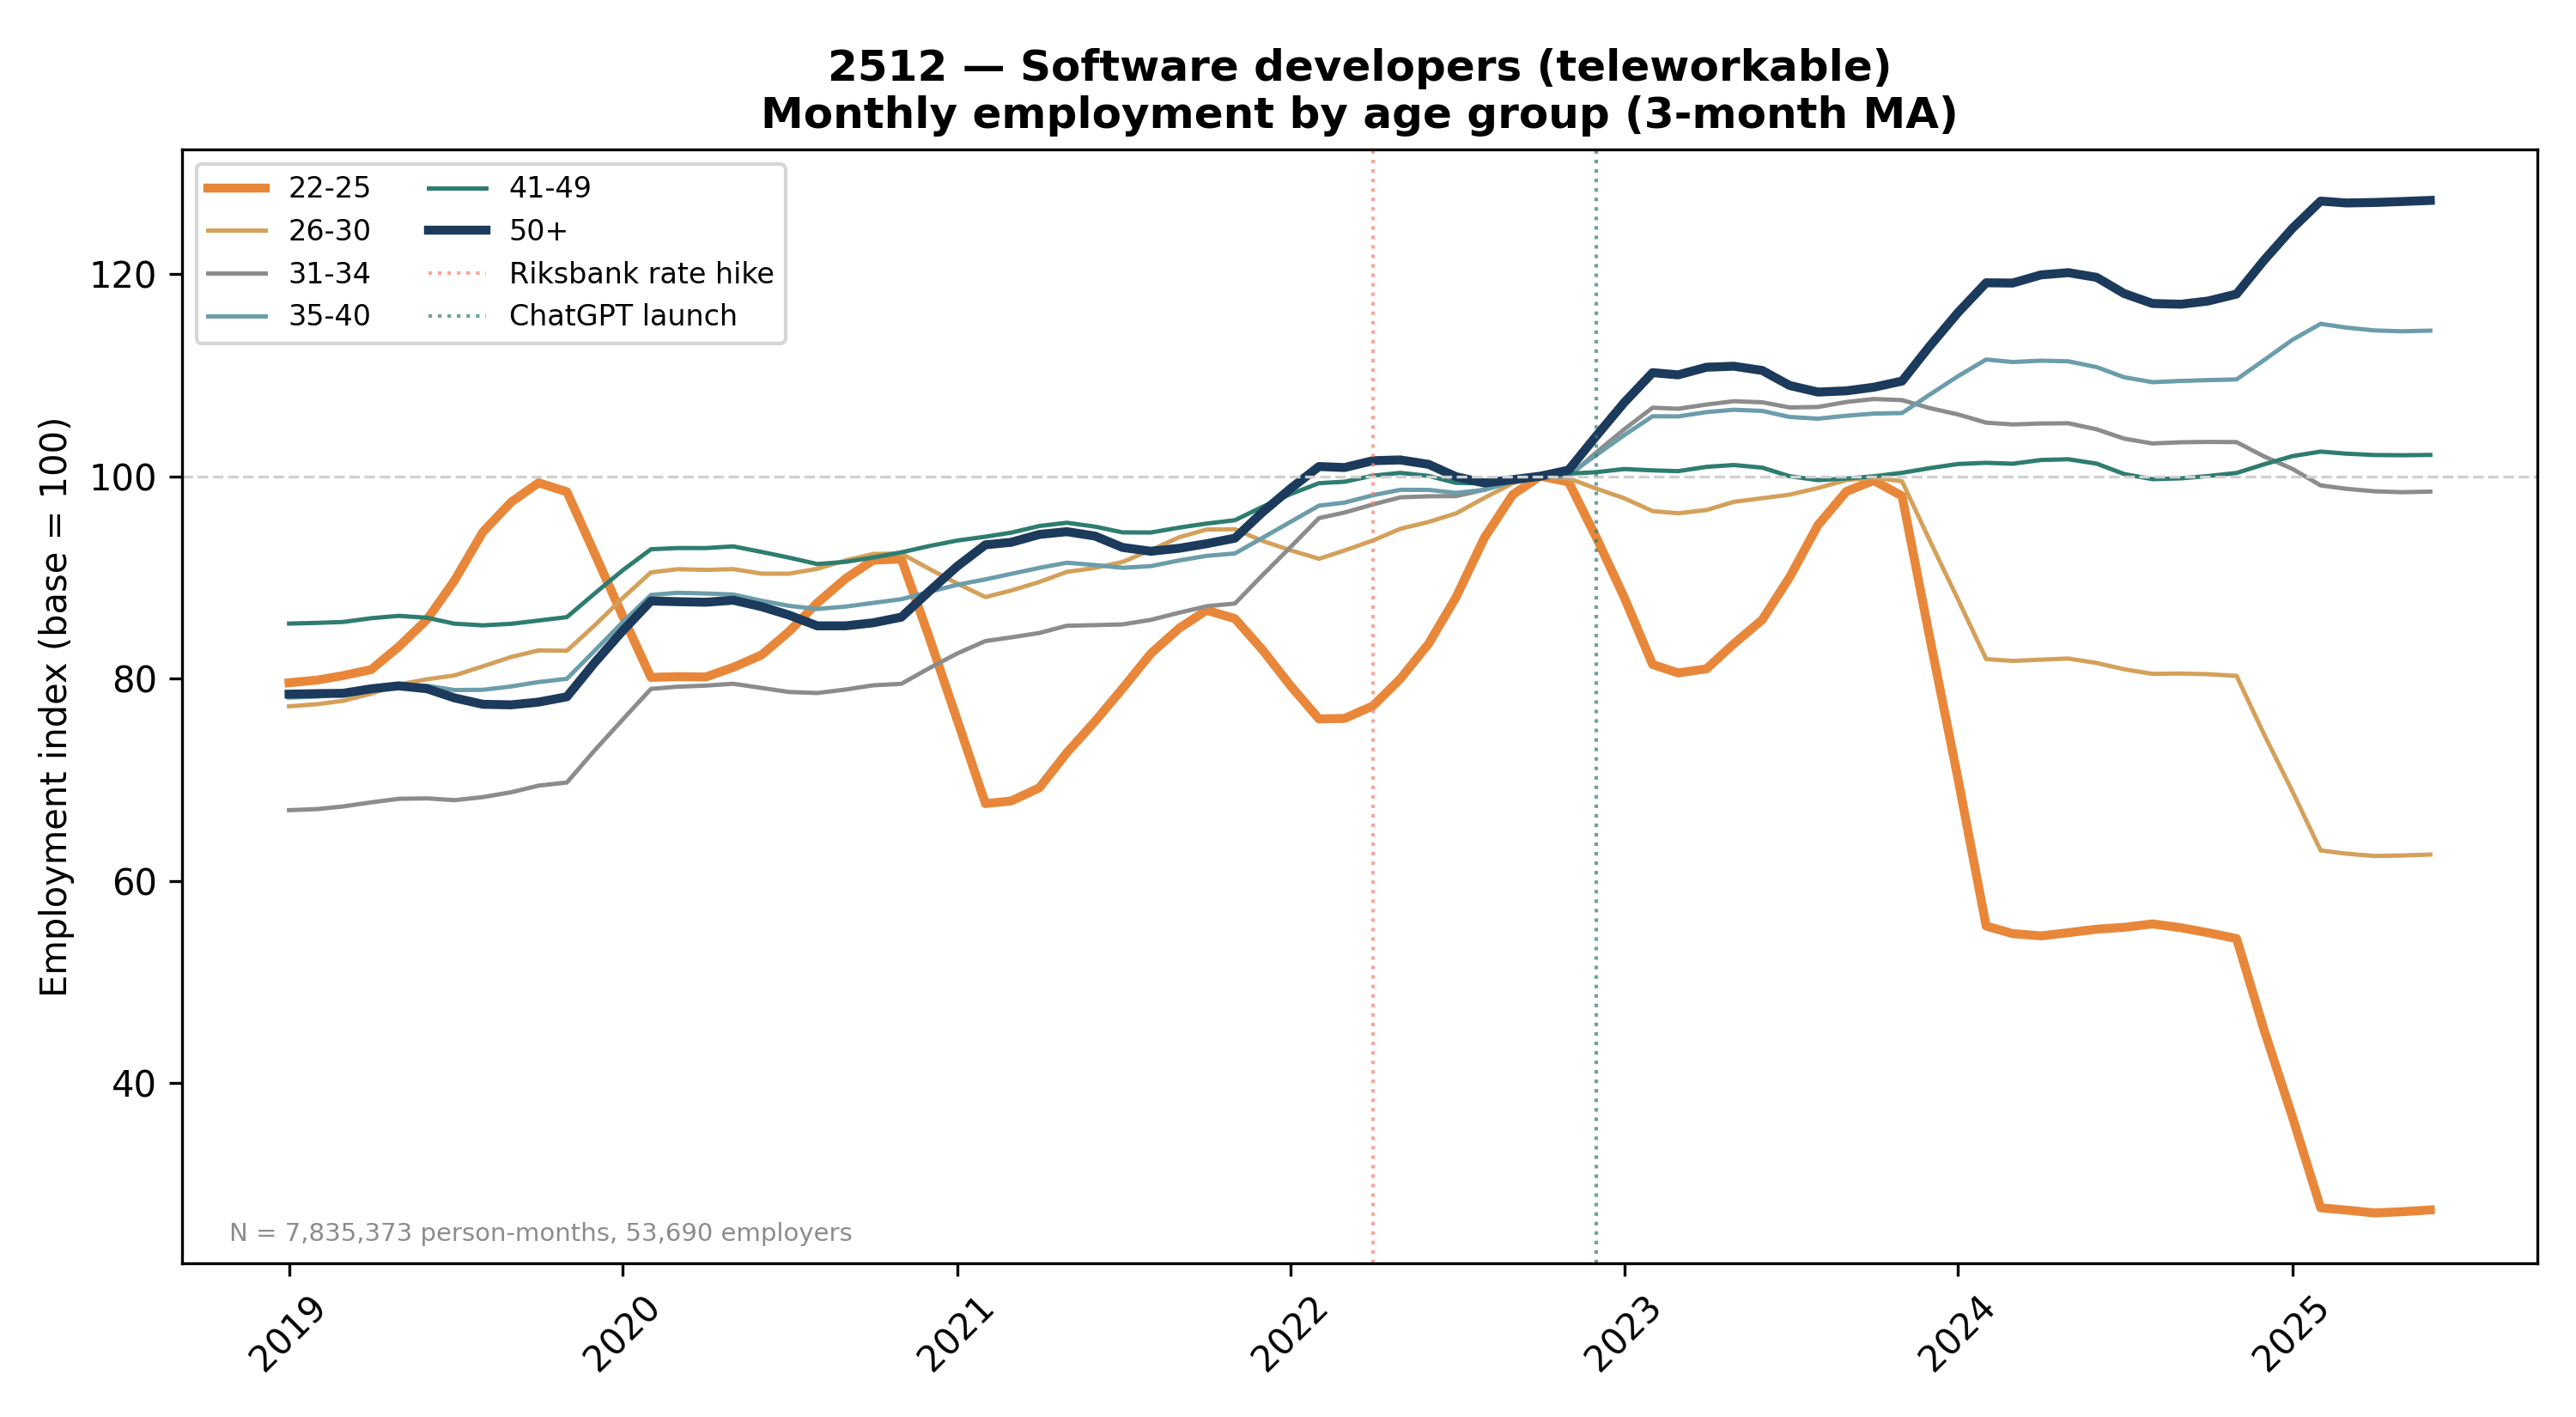
\includegraphics[width=\textwidth]{figA8a_mona_canaries_softwaredevelopers.png}\\[-1mm]
\footnotesize Software developers (SSYK 2512)
\vspace{1mm}
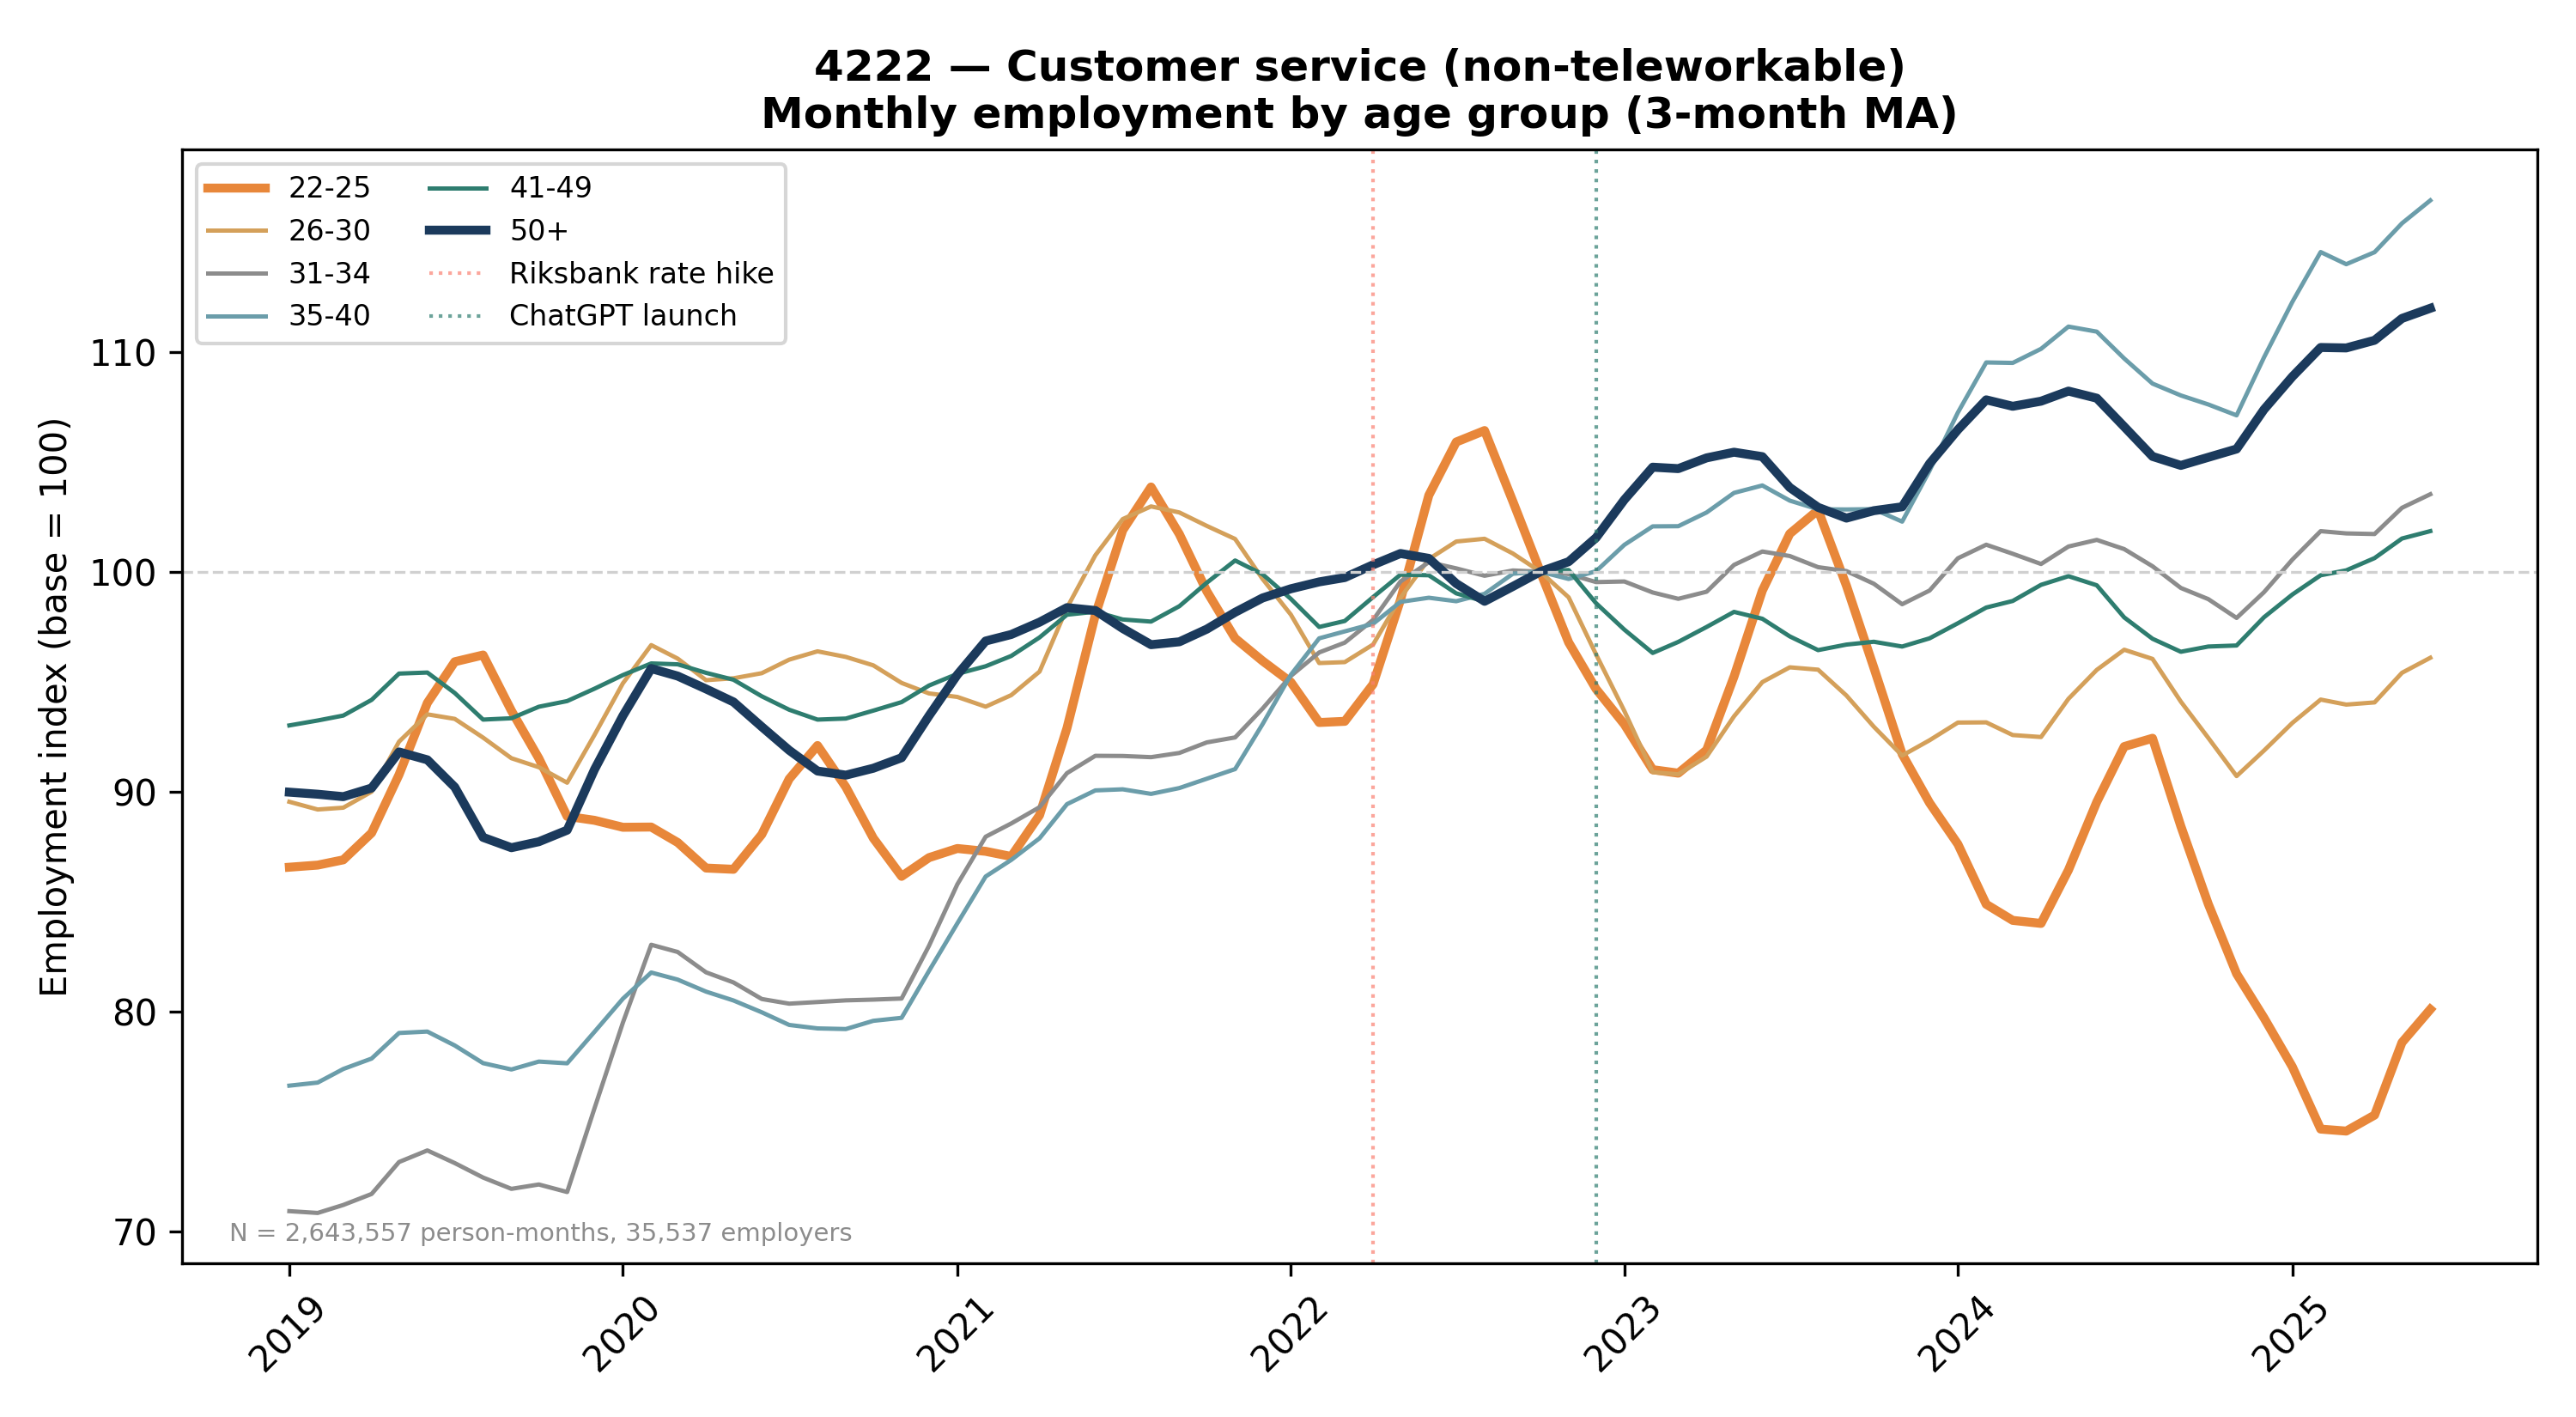
\includegraphics[width=\textwidth]{figA8b_mona_canaries_customerservice.png}\\[-1mm]
\footnotesize Customer service (SSYK 4221/4222)
\end{column}
\begin{column}{0.48\textwidth}
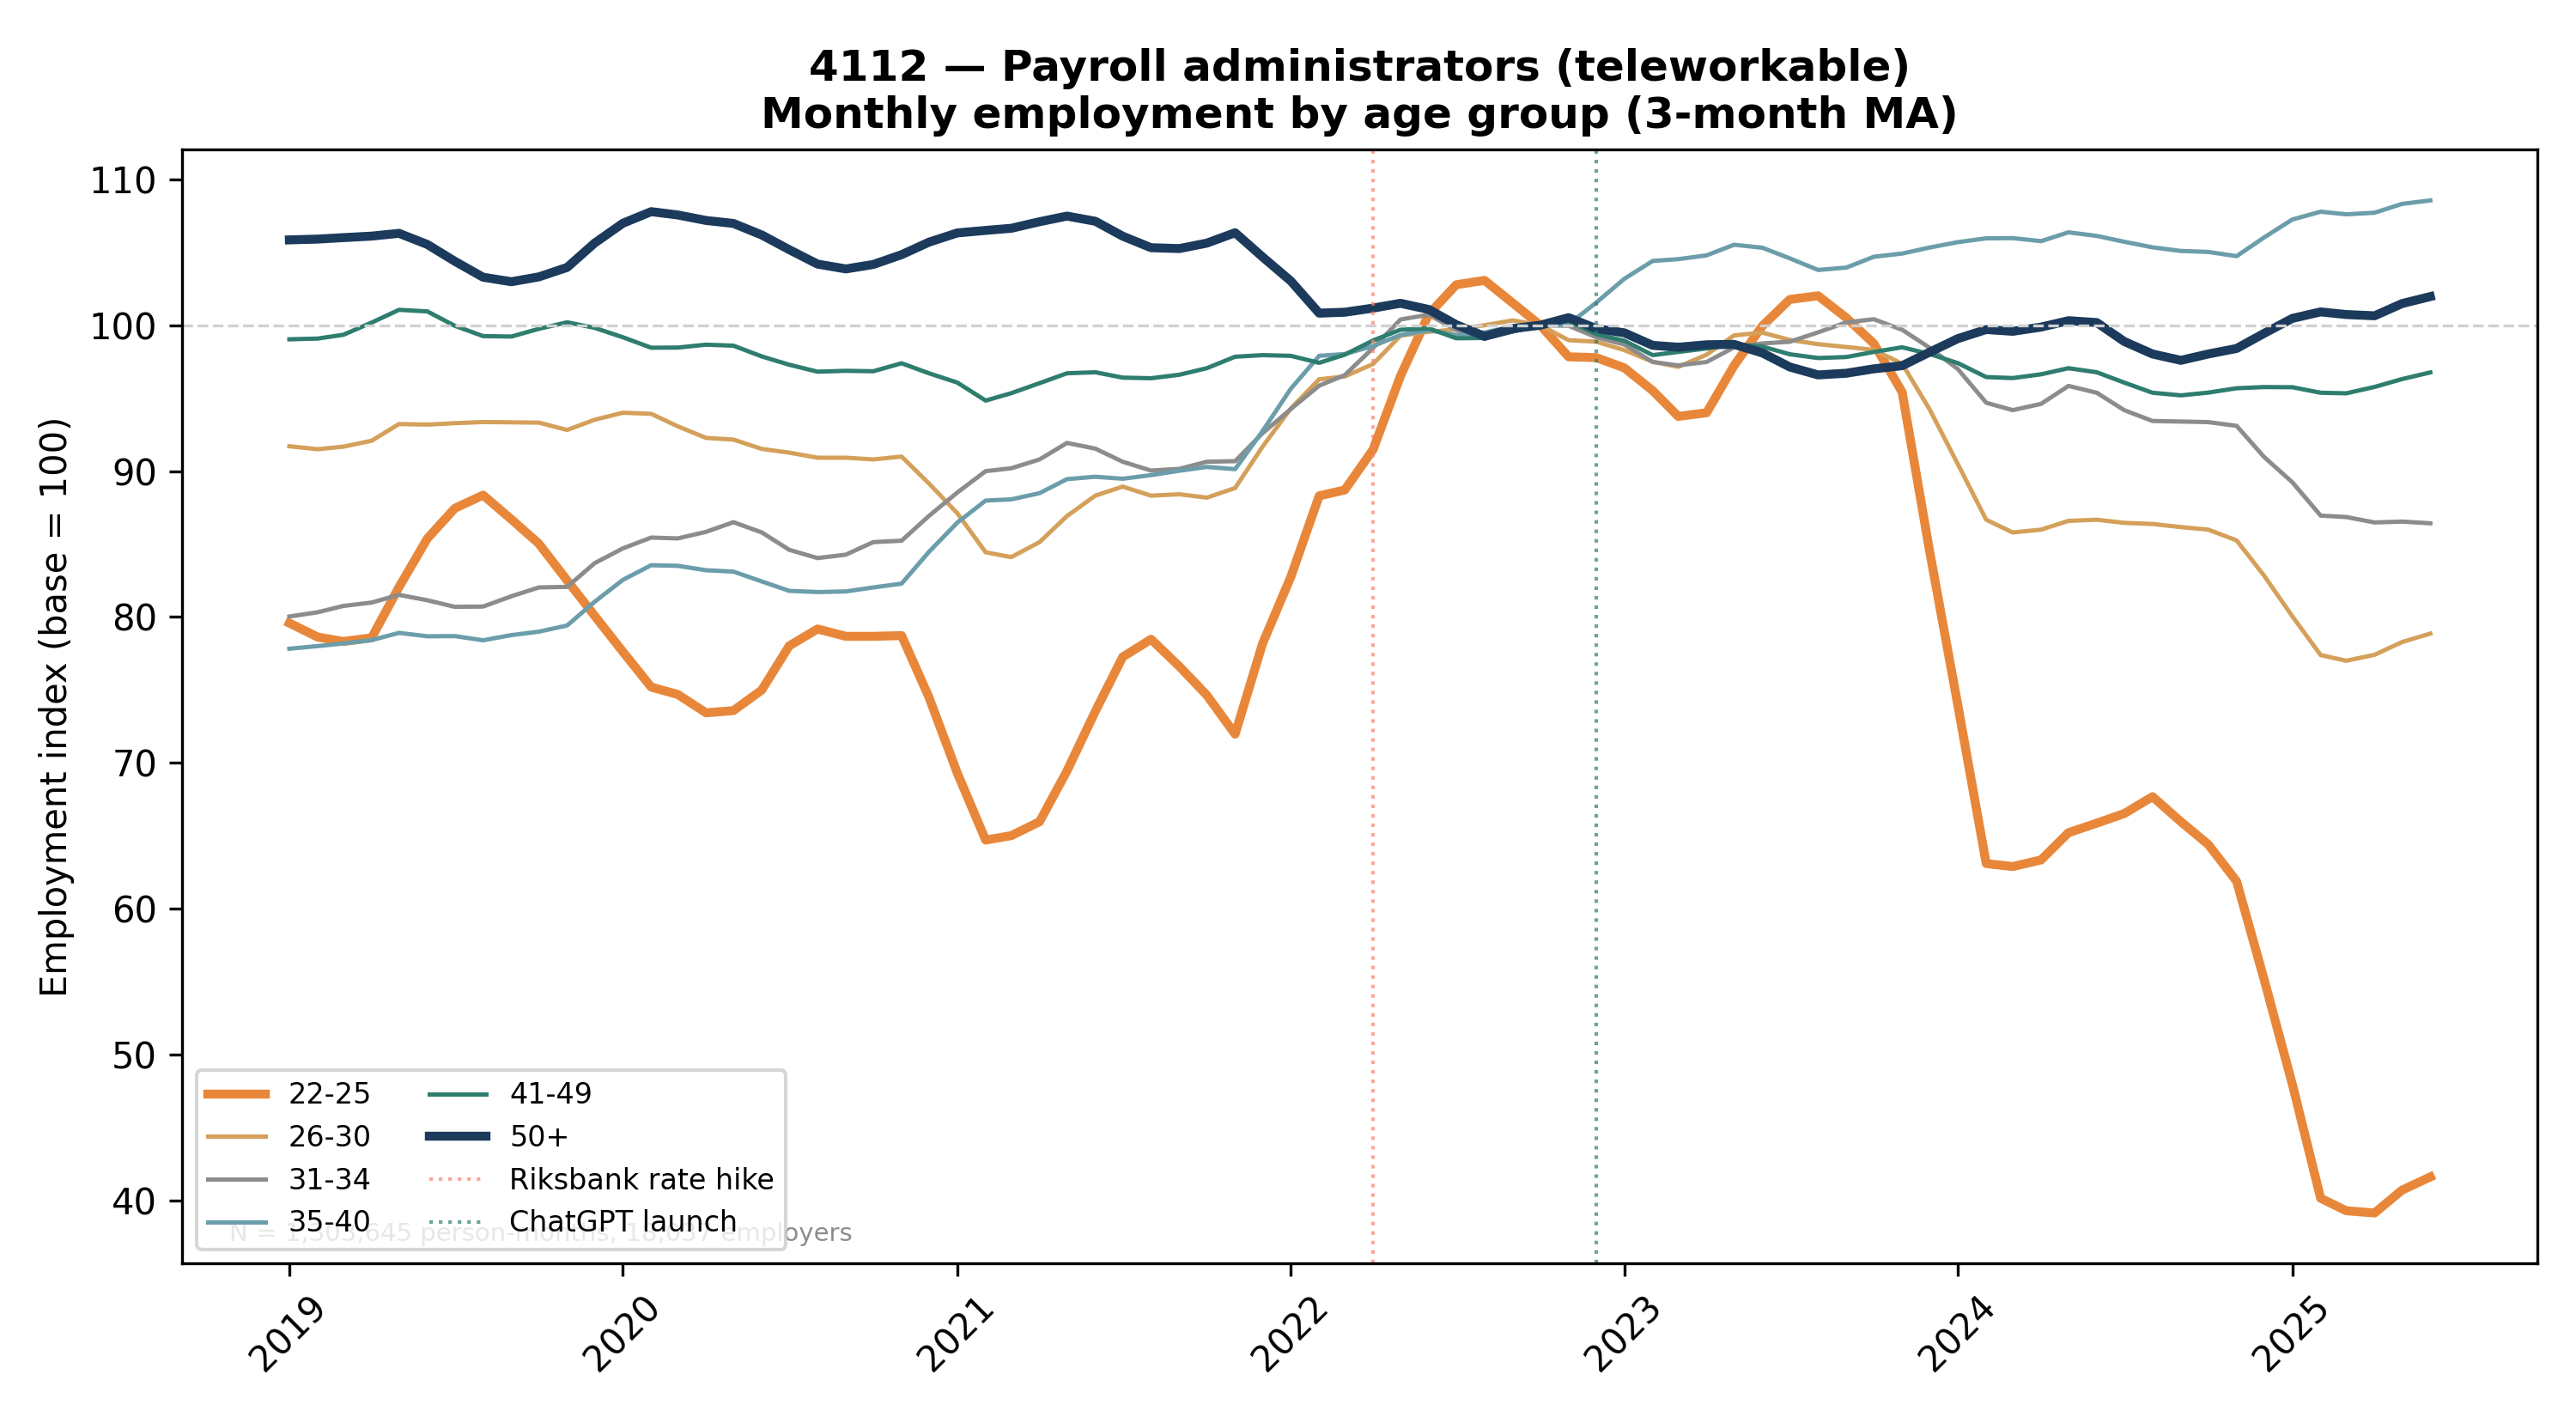
\includegraphics[width=\textwidth]{figA8c_mona_canaries_payrolladmin.png}\\[-1mm]
\footnotesize Payroll administrators (SSYK 4112)
\vspace{1mm}
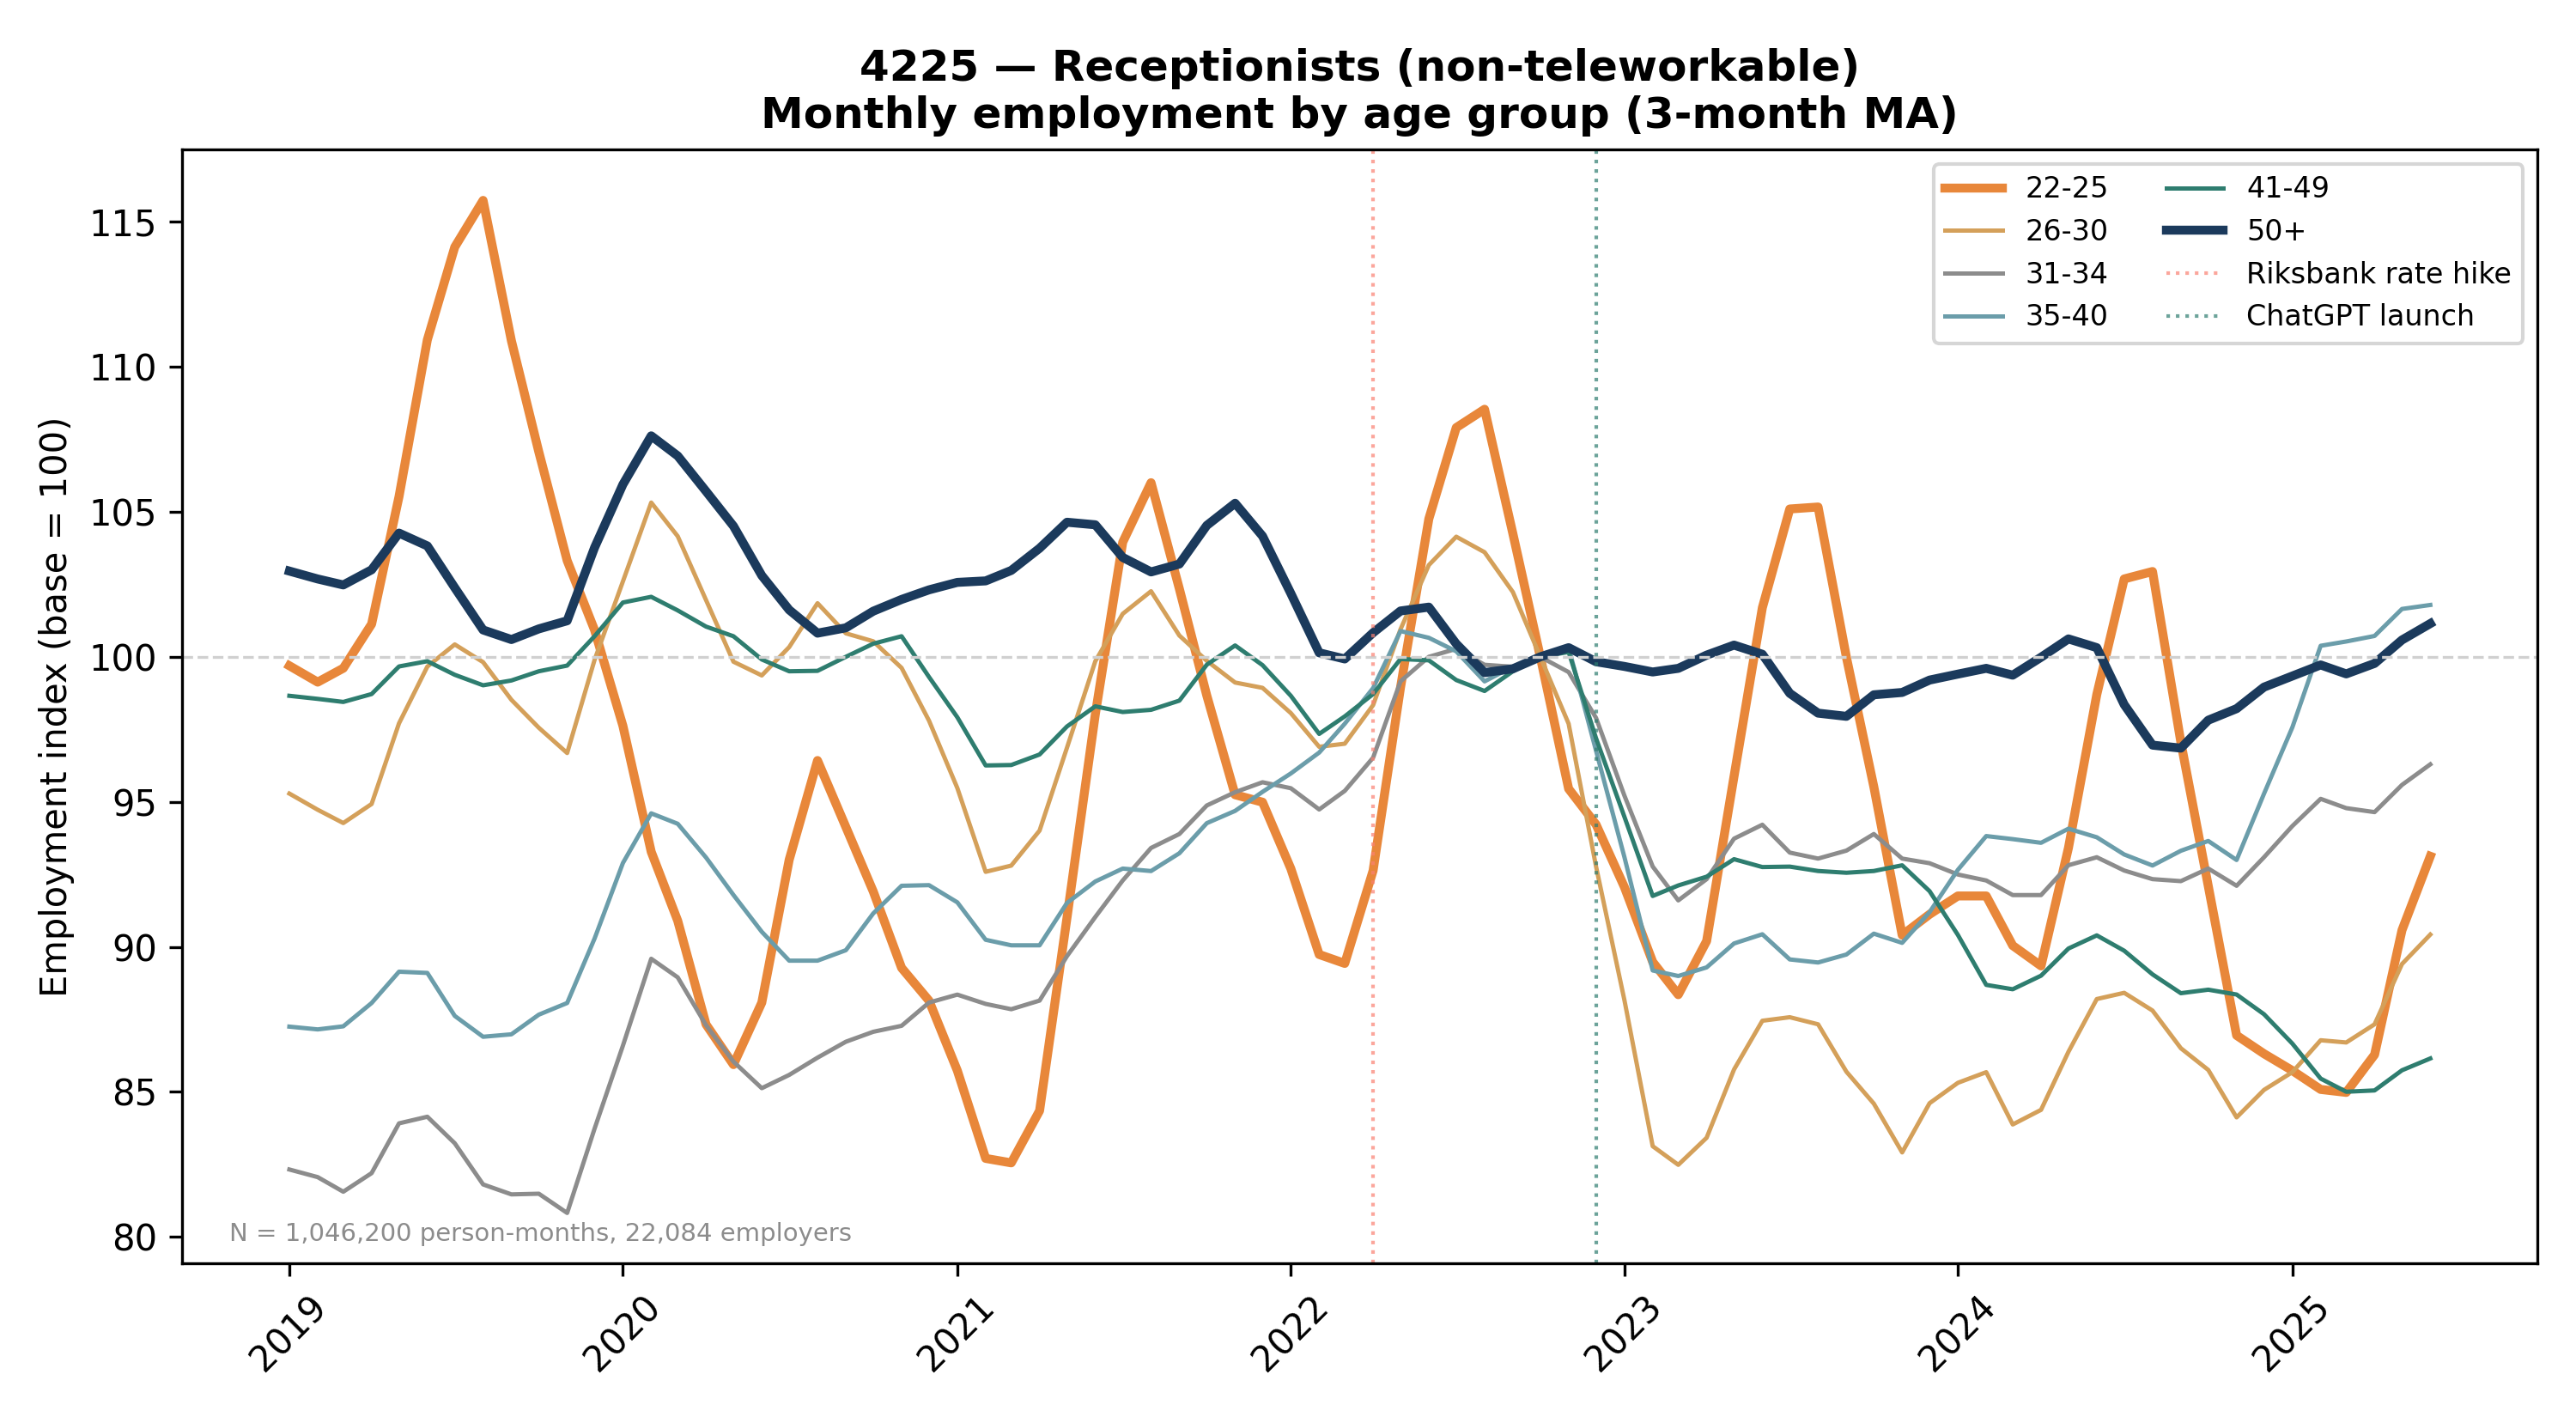
\includegraphics[width=\textwidth]{figA8d_mona_canaries_receptionists.png}\\[-1mm]
\footnotesize Receptionists (SSYK 4225)
\end{column}
\end{columns}
\vspace{1mm}
\hfill{\tiny\hyperlink{main:daioe}{\beamerreturnbutton{Back}}}
\end{frame}

\begin{frame}{Riksbank policy rate timeline}
\hypertarget{backup:riksbank}{}
\begin{center}
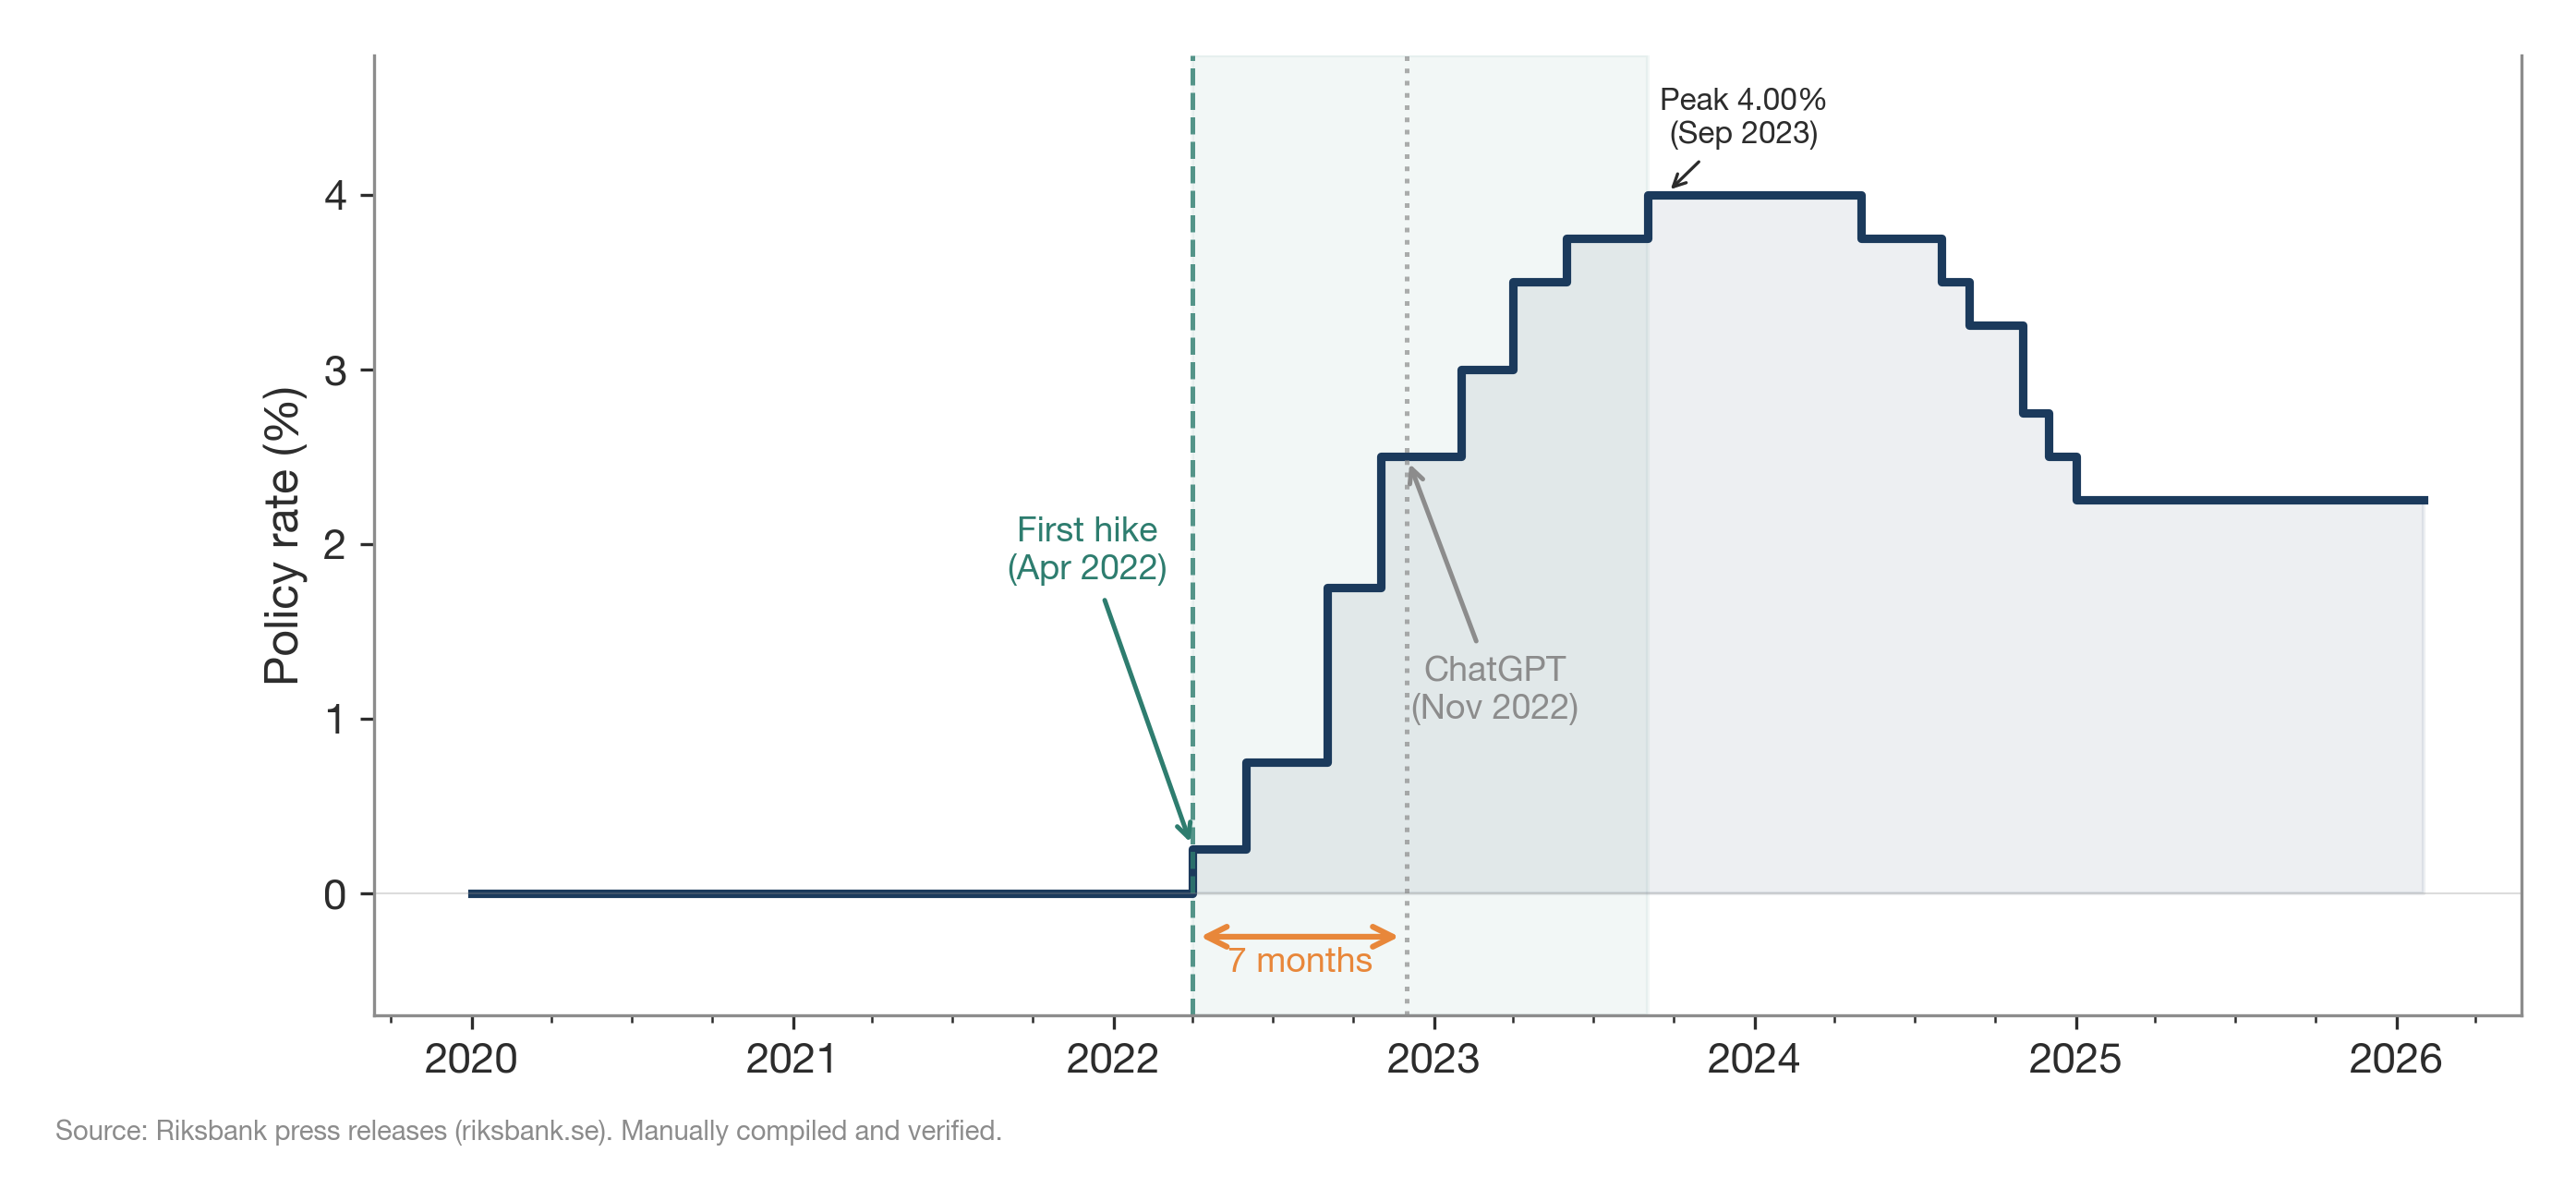
\includegraphics[width=0.7\textwidth]{figA10_riksbank_rate.png}
\end{center}
\footnotesize Riksbank policy rate, 2020--2026. First hike: April 2022. ChatGPT launch: November 2022. Seven-month gap exploited for timing identification.
\hfill{\tiny\hyperlink{main:scarychart}{\beamerreturnbutton{Back}}}
\end{frame}

\begin{frame}{Extensive margin: zero-cell shares}
\hypertarget{backup:extensive}{}
\begin{center}
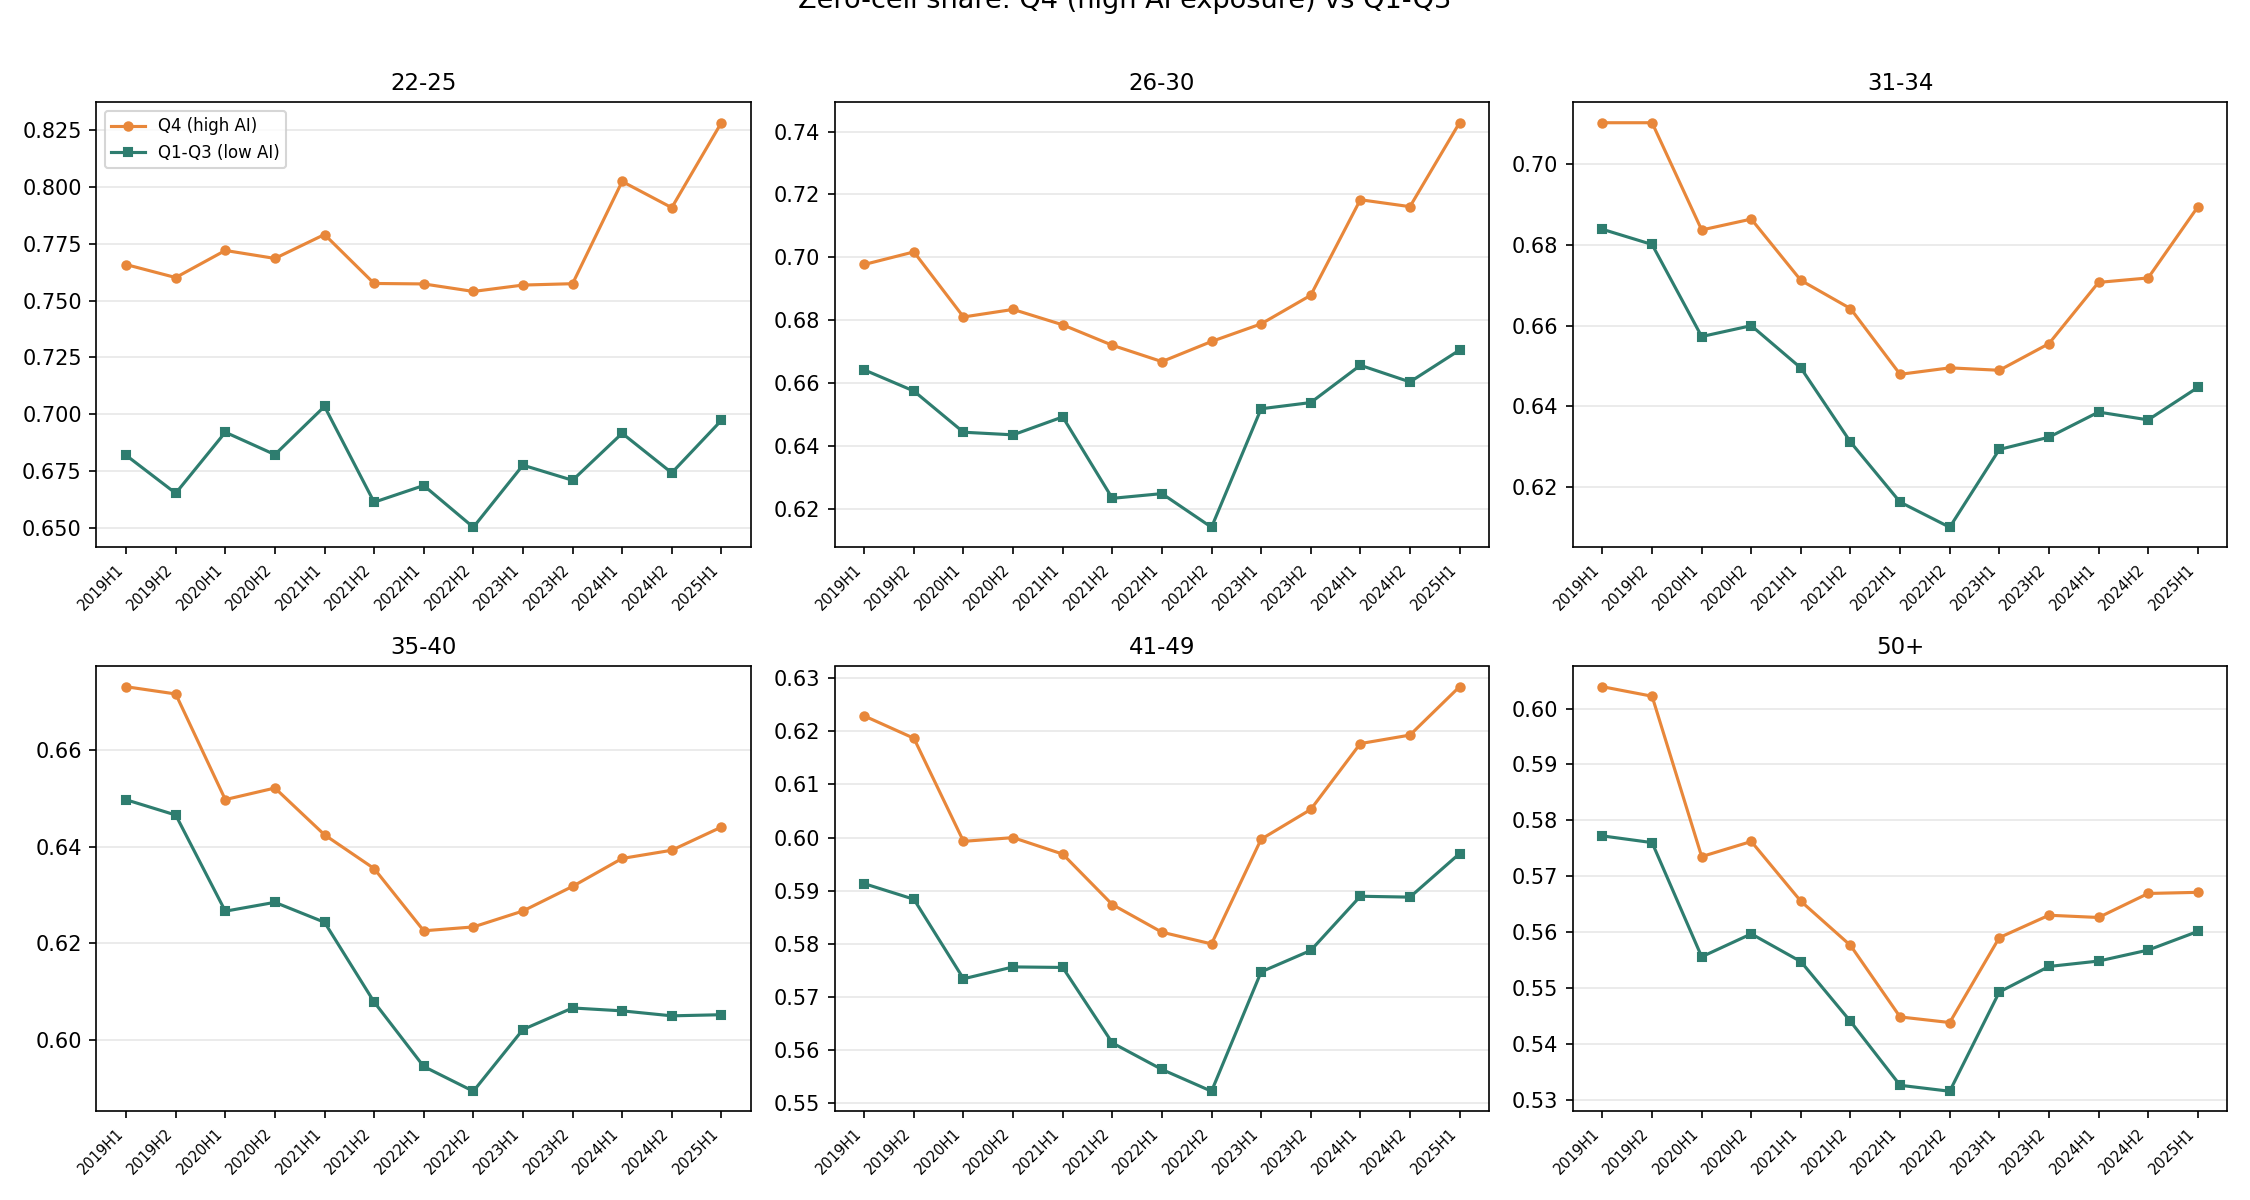
\includegraphics[width=0.7\textwidth]{zero_cell_shares_q4_vs_rest.png}
\end{center}
\footnotesize Share of employer $\times$ occupation cells with zero employment. Young workers (22--25) in Q4 occupations increasingly absent from employer rosters; opposite for 50+.
\hfill{\tiny\hyperlink{main:daioe}{\beamerreturnbutton{Back}}}
\end{frame}

\begin{frame}{Event studies by age group}
\begin{center}
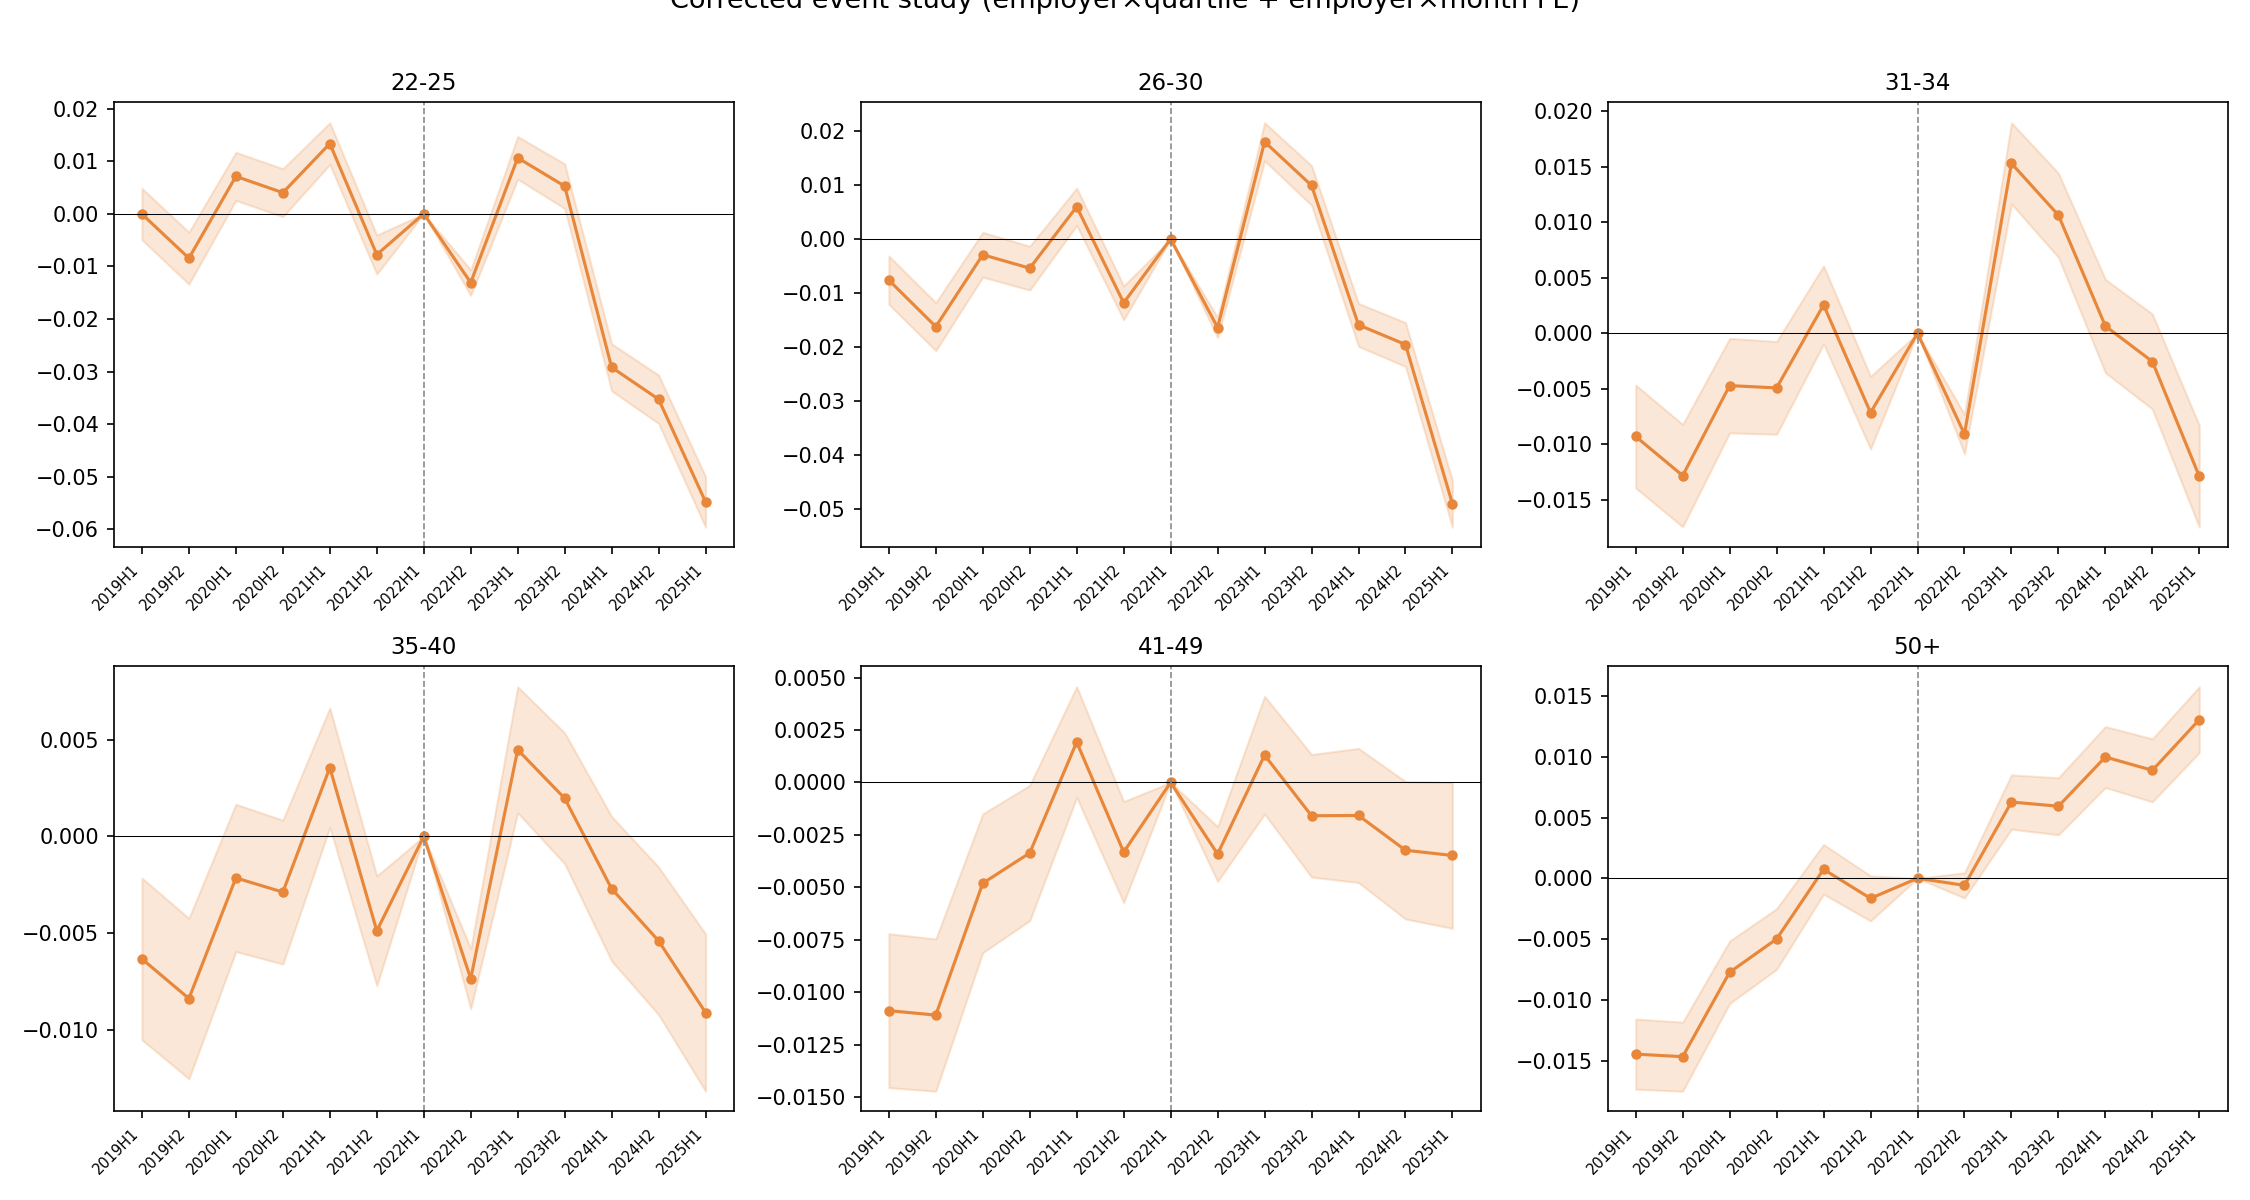
\includegraphics[width=0.85\textwidth]{corrected_es_panel.png}
\end{center}
\vspace{-3mm}
\footnotesize Employer $\times$ quartile FE + employer $\times$ month FE. 95\% CIs. Vertical line: ChatGPT (Nov 2022).
\end{frame}

\end{document}
